\documentclass[twoside]{book}

% Packages required by doxygen
\usepackage{fixltx2e}
\usepackage{calc}
\usepackage{doxygen}
\usepackage[export]{adjustbox} % also loads graphicx
\usepackage{graphicx}
\usepackage[utf8]{inputenc}
\usepackage{makeidx}
\usepackage{multicol}
\usepackage{multirow}
\PassOptionsToPackage{warn}{textcomp}
\usepackage{textcomp}
\usepackage[nointegrals]{wasysym}
\usepackage[table]{xcolor}

% Font selection
\usepackage[T1]{fontenc}
\usepackage[scaled=.90]{helvet}
\usepackage{courier}
\usepackage{amssymb}
\usepackage{sectsty}
\renewcommand{\familydefault}{\sfdefault}
\allsectionsfont{%
  \fontseries{bc}\selectfont%
  \color{darkgray}%
}
\renewcommand{\DoxyLabelFont}{%
  \fontseries{bc}\selectfont%
  \color{darkgray}%
}
\newcommand{\+}{\discretionary{\mbox{\scriptsize$\hookleftarrow$}}{}{}}

% Page & text layout
\usepackage{geometry}
\geometry{%
  a4paper,%
  top=2.5cm,%
  bottom=2.5cm,%
  left=2.5cm,%
  right=2.5cm%
}
\tolerance=750
\hfuzz=15pt
\hbadness=750
\setlength{\emergencystretch}{15pt}
\setlength{\parindent}{0cm}
\setlength{\parskip}{0.2cm}
\makeatletter
\renewcommand{\paragraph}{%
  \@startsection{paragraph}{4}{0ex}{-1.0ex}{1.0ex}{%
    \normalfont\normalsize\bfseries\SS@parafont%
  }%
}
\renewcommand{\subparagraph}{%
  \@startsection{subparagraph}{5}{0ex}{-1.0ex}{1.0ex}{%
    \normalfont\normalsize\bfseries\SS@subparafont%
  }%
}
\makeatother

% Headers & footers
\usepackage{fancyhdr}
\pagestyle{fancyplain}
\fancyhead[LE]{\fancyplain{}{\bfseries\thepage}}
\fancyhead[CE]{\fancyplain{}{}}
\fancyhead[RE]{\fancyplain{}{\bfseries\leftmark}}
\fancyhead[LO]{\fancyplain{}{\bfseries\rightmark}}
\fancyhead[CO]{\fancyplain{}{}}
\fancyhead[RO]{\fancyplain{}{\bfseries\thepage}}
\fancyfoot[LE]{\fancyplain{}{}}
\fancyfoot[CE]{\fancyplain{}{}}
\fancyfoot[RE]{\fancyplain{}{\bfseries\scriptsize Generated on Thu Oct 22 2015 09\+:51\+:50 for My Project by Doxygen }}
\fancyfoot[LO]{\fancyplain{}{\bfseries\scriptsize Generated on Thu Oct 22 2015 09\+:51\+:50 for My Project by Doxygen }}
\fancyfoot[CO]{\fancyplain{}{}}
\fancyfoot[RO]{\fancyplain{}{}}
\renewcommand{\footrulewidth}{0.4pt}
\renewcommand{\chaptermark}[1]{%
  \markboth{#1}{}%
}
\renewcommand{\sectionmark}[1]{%
  \markright{\thesection\ #1}%
}

% Indices & bibliography
\usepackage{natbib}
\usepackage[titles]{tocloft}
\setcounter{tocdepth}{3}
\setcounter{secnumdepth}{5}
\makeindex

% Hyperlinks (required, but should be loaded last)
\usepackage{ifpdf}
\ifpdf
  \usepackage[pdftex,pagebackref=true]{hyperref}
\else
  \usepackage[ps2pdf,pagebackref=true]{hyperref}
\fi
\hypersetup{%
  colorlinks=true,%
  linkcolor=blue,%
  citecolor=blue,%
  unicode%
}

% Custom commands
\newcommand{\clearemptydoublepage}{%
  \newpage{\pagestyle{empty}\cleardoublepage}%
}


%===== C O N T E N T S =====

\begin{document}

% Titlepage & ToC
\hypersetup{pageanchor=false,
             bookmarks=true,
             bookmarksnumbered=true,
             pdfencoding=unicode
            }
\pagenumbering{roman}
\begin{titlepage}
\vspace*{7cm}
\begin{center}%
{\Large My Project }\\
\vspace*{1cm}
{\large Generated by Doxygen 1.8.10}\\
\vspace*{0.5cm}
{\small Thu Oct 22 2015 09:51:50}\\
\end{center}
\end{titlepage}
\clearemptydoublepage
\tableofcontents
\clearemptydoublepage
\pagenumbering{arabic}
\hypersetup{pageanchor=true}

%--- Begin generated contents ---
\chapter{Hierarchical Index}
\section{Class Hierarchy}
This inheritance list is sorted roughly, but not completely, alphabetically\+:\begin{DoxyCompactList}
\item \contentsline{section}{Double\+Position}{\pageref{class_double_position}}{}
\item \contentsline{section}{Firework}{\pageref{class_firework}}{}
\item \contentsline{section}{Ghost\+Timer}{\pageref{class_ghost_timer}}{}
\item \contentsline{section}{Grid}{\pageref{class_grid}}{}
\item Q\+Object\begin{DoxyCompactList}
\item \contentsline{section}{Arduino\+Handler}{\pageref{class_arduino_handler}}{}
\item \contentsline{section}{Game}{\pageref{class_game}}{}
\item \contentsline{section}{Level}{\pageref{class_level}}{}
\item \contentsline{section}{Pacman\+Unit}{\pageref{class_pacman_unit}}{}
\end{DoxyCompactList}
\item Q\+Widget\begin{DoxyCompactList}
\item \contentsline{section}{Pacscreen}{\pageref{class_pacscreen}}{}
\end{DoxyCompactList}
\item \contentsline{section}{Texture\+Handler}{\pageref{class_texture_handler}}{}
\item \contentsline{section}{Unit}{\pageref{class_unit}}{}
\begin{DoxyCompactList}
\item \contentsline{section}{Ghost}{\pageref{class_ghost}}{}
\item \contentsline{section}{Pacman\+Unit}{\pageref{class_pacman_unit}}{}
\end{DoxyCompactList}
\end{DoxyCompactList}

\chapter{Class Index}
\section{Class List}
Here are the classes, structs, unions and interfaces with brief descriptions\+:\begin{DoxyCompactList}
\item\contentsline{section}{\hyperlink{class_editor_game}{Editor\+Game} \\*La classe \hyperlink{class_editor_game}{Editor\+Game} gère l\textquotesingle{}ensemble des paramètres pouvant être passés au programme Pacman }{\pageref{class_editor_game}}{}
\item\contentsline{section}{\hyperlink{class_editor_level}{Editor\+Level} \\*La classe \hyperlink{class_editor_level}{Editor\+Level} permet de paramétrer un niveau dans Pacman }{\pageref{class_editor_level}}{}
\item\contentsline{section}{\hyperlink{class_editor_unit}{Editor\+Unit} \\*Petite classe graphique permettant de bouger un pion }{\pageref{class_editor_unit}}{}
\item\contentsline{section}{\hyperlink{class_ghost_timer}{Ghost\+Timer} \\*Classe de Timer pour les modes des fantômes }{\pageref{class_ghost_timer}}{}
\item\contentsline{section}{\hyperlink{class_main_window}{Main\+Window} \\*Classe principale graphique }{\pageref{class_main_window}}{}
\item\contentsline{section}{\hyperlink{class_map}{Map} \\*Objet graphique détectant les clics souris et générant des signaux }{\pageref{class_map}}{}
\item\contentsline{section}{\hyperlink{class_new_ghost_mode_dialog}{New\+Ghost\+Mode\+Dialog} \\*Classe graphique de fenêtre pour l\textquotesingle{}ajout d\textquotesingle{}un nouveau mode de poursuite }{\pageref{class_new_ghost_mode_dialog}}{}
\item\contentsline{section}{\hyperlink{class_new_level_dialog}{New\+Level\+Dialog} \\*Classe graphique de fenêtre pour l\textquotesingle{}ajout d\textquotesingle{}un nouveau niveaau }{\pageref{class_new_level_dialog}}{}
\item\contentsline{section}{\hyperlink{class_texture_handler}{Texture\+Handler} \\*Gestionnaire de textures }{\pageref{class_texture_handler}}{}
\item\contentsline{section}{\hyperlink{class_texture_select_dialog}{Texture\+Select\+Dialog} \\*Classe de fenêtre de sélection de texture }{\pageref{class_texture_select_dialog}}{}
\item\contentsline{section}{\hyperlink{struct_unit_data__str}{Unit\+Data\+\_\+str} \\*Petite structure regroupant les paramètres principaux d\textquotesingle{}une unité }{\pageref{struct_unit_data__str}}{}
\item\contentsline{section}{\hyperlink{structunit_widget_set__str}{unit\+Widget\+Set\+\_\+str} \\*Structure contenant les objets d\textquotesingle{}interface lié à une unité }{\pageref{structunit_widget_set__str}}{}
\item\contentsline{section}{\hyperlink{class_view}{View} \\*Classe graphique remplaçant la vue de Qt pour propager les événements }{\pageref{class_view}}{}
\end{DoxyCompactList}

\chapter{Class Documentation}
\hypertarget{class_editor_game}{}\section{Editor\+Game Class Reference}
\label{class_editor_game}\index{Editor\+Game@{Editor\+Game}}


La classe \hyperlink{class_editor_game}{Editor\+Game} gère l\textquotesingle{}ensemble des paramètres pouvant être passés au programme Pacman.  




{\ttfamily \#include $<$editorgame.\+h$>$}

\subsection*{Public Member Functions}
\begin{DoxyCompactItemize}
\item 
\hyperlink{class_editor_game_a81d7f33e9c0f5ce417db16ac121c3ca7}{Editor\+Game} ()
\begin{DoxyCompactList}\small\item\em Constructeur de base de \hyperlink{class_editor_game}{Editor\+Game}. \end{DoxyCompactList}\item 
\hyperlink{class_editor_game_aa39c9fa83c78da05b03477ac172c03e6}{Editor\+Game} (Q\+Dom\+Document dom)
\begin{DoxyCompactList}\small\item\em Constructeur X\+M\+L de \hyperlink{class_editor_game}{Editor\+Game}. \end{DoxyCompactList}\item 
\hyperlink{class_editor_game_a910df7a6be24a5ab77f51ab04bfa2a64}{$\sim$\+Editor\+Game} ()
\begin{DoxyCompactList}\small\item\em Destructeur de \hyperlink{class_editor_game}{Editor\+Game}. \end{DoxyCompactList}\item 
\hyperlink{class_editor_level}{Editor\+Level} $\ast$ \hyperlink{class_editor_game_a071f3a0c8398c26e3d8ffcd8f38f71df}{level} (int index) const 
\begin{DoxyCompactList}\small\item\em Getter. \end{DoxyCompactList}\item 
void \hyperlink{class_editor_game_a08a34b285392ce950141e92e8a3e2490}{add\+Level} (\hyperlink{class_editor_level}{Editor\+Level} $\ast$\hyperlink{class_editor_game_a071f3a0c8398c26e3d8ffcd8f38f71df}{level})
\begin{DoxyCompactList}\small\item\em Ajoute un niveau à l\textquotesingle{}objet. \end{DoxyCompactList}\item 
int \hyperlink{class_editor_game_a84465e0451cf75b8732630452263584c}{levels\+Count} () const 
\begin{DoxyCompactList}\small\item\em Getter. \end{DoxyCompactList}\item 
int \hyperlink{class_editor_game_afb6b6a5ac54114f098d840592f64c6cb}{texture\+Count} () const 
\begin{DoxyCompactList}\small\item\em Getter. \end{DoxyCompactList}\item 
\hyperlink{class_texture_handler}{Texture\+Handler} $\ast$ \hyperlink{class_editor_game_acc719e48b13201125f52dbddb530e77e}{texture\+Handler} ()
\begin{DoxyCompactList}\small\item\em Getter. \end{DoxyCompactList}\item 
void \hyperlink{class_editor_game_a181792868a77319e18860e4887a15bd3}{save} (Q\+String filename) const 
\begin{DoxyCompactList}\small\item\em Sauvegarde l\textquotesingle{}ensemble des paramètres dans le fichier donné. \end{DoxyCompactList}\end{DoxyCompactItemize}


\subsection{Detailed Description}
La classe \hyperlink{class_editor_game}{Editor\+Game} gère l\textquotesingle{}ensemble des paramètres pouvant être passés au programme Pacman. 

\begin{DoxyAuthor}{Author}
Valentin D.\+d.\+G. 
\end{DoxyAuthor}
\begin{DoxyVersion}{Version}
1.\+0
\end{DoxyVersion}
La classe gère un ensemble de niveaux dont les paramètres sont via une U\+I. \hyperlink{class_editor_game}{Editor\+Game} peut s\textquotesingle{}instancier avec un document X\+M\+L et s\textquotesingle{}exporter de la même façon afin de sauvegarder les données. 

\subsection{Constructor \& Destructor Documentation}
\hypertarget{class_editor_game_a81d7f33e9c0f5ce417db16ac121c3ca7}{}\index{Editor\+Game@{Editor\+Game}!Editor\+Game@{Editor\+Game}}
\index{Editor\+Game@{Editor\+Game}!Editor\+Game@{Editor\+Game}}
\subsubsection[{Editor\+Game()}]{\setlength{\rightskip}{0pt plus 5cm}Editor\+Game\+::\+Editor\+Game (
\begin{DoxyParamCaption}
{}
\end{DoxyParamCaption}
)}\label{class_editor_game_a81d7f33e9c0f5ce417db16ac121c3ca7}


Constructeur de base de \hyperlink{class_editor_game}{Editor\+Game}. 

Crée une instance de \hyperlink{class_editor_game}{Editor\+Game} vide qui ne dispose d\textquotesingle{}aucun niveau ni d\textquotesingle{}aucun paramètres. Lors de cette instanciation, le gestionnaire de texture est créé afin d\textquotesingle{}être utilisé par l\textquotesingle{}ensemble des niveaux. \hypertarget{class_editor_game_aa39c9fa83c78da05b03477ac172c03e6}{}\index{Editor\+Game@{Editor\+Game}!Editor\+Game@{Editor\+Game}}
\index{Editor\+Game@{Editor\+Game}!Editor\+Game@{Editor\+Game}}
\subsubsection[{Editor\+Game(\+Q\+Dom\+Document dom)}]{\setlength{\rightskip}{0pt plus 5cm}Editor\+Game\+::\+Editor\+Game (
\begin{DoxyParamCaption}
\item[{Q\+Dom\+Document}]{dom}
\end{DoxyParamCaption}
)}\label{class_editor_game_aa39c9fa83c78da05b03477ac172c03e6}


Constructeur X\+M\+L de \hyperlink{class_editor_game}{Editor\+Game}. 


\begin{DoxyParams}{Parameters}
{\em dom} & Document X\+M\+L contenant les paramètres sauvegardés.\\
\hline
\end{DoxyParams}
Crée une instance de \hyperlink{class_editor_game}{Editor\+Game} qui charge les paramètres se trouvant dans le document X\+M\+L. \hypertarget{class_editor_game_a910df7a6be24a5ab77f51ab04bfa2a64}{}\index{Editor\+Game@{Editor\+Game}!````~Editor\+Game@{$\sim$\+Editor\+Game}}
\index{````~Editor\+Game@{$\sim$\+Editor\+Game}!Editor\+Game@{Editor\+Game}}
\subsubsection[{$\sim$\+Editor\+Game()}]{\setlength{\rightskip}{0pt plus 5cm}Editor\+Game\+::$\sim$\+Editor\+Game (
\begin{DoxyParamCaption}
{}
\end{DoxyParamCaption}
)}\label{class_editor_game_a910df7a6be24a5ab77f51ab04bfa2a64}


Destructeur de \hyperlink{class_editor_game}{Editor\+Game}. 

Désalloue la mémoire de l\textquotesingle{}objet en plus de celles des niveaux qu\textquotesingle{}il contient. 

\subsection{Member Function Documentation}
\hypertarget{class_editor_game_a08a34b285392ce950141e92e8a3e2490}{}\index{Editor\+Game@{Editor\+Game}!add\+Level@{add\+Level}}
\index{add\+Level@{add\+Level}!Editor\+Game@{Editor\+Game}}
\subsubsection[{add\+Level(\+Editor\+Level $\ast$level)}]{\setlength{\rightskip}{0pt plus 5cm}void Editor\+Game\+::add\+Level (
\begin{DoxyParamCaption}
\item[{{\bf Editor\+Level} $\ast$}]{level}
\end{DoxyParamCaption}
)}\label{class_editor_game_a08a34b285392ce950141e92e8a3e2490}


Ajoute un niveau à l\textquotesingle{}objet. 


\begin{DoxyParams}{Parameters}
{\em level} & Pointeur sur le niveau ajouté. \\
\hline
\end{DoxyParams}
\hypertarget{class_editor_game_a071f3a0c8398c26e3d8ffcd8f38f71df}{}\index{Editor\+Game@{Editor\+Game}!level@{level}}
\index{level@{level}!Editor\+Game@{Editor\+Game}}
\subsubsection[{level(int index) const }]{\setlength{\rightskip}{0pt plus 5cm}{\bf Editor\+Level} $\ast$ Editor\+Game\+::level (
\begin{DoxyParamCaption}
\item[{int}]{index}
\end{DoxyParamCaption}
) const}\label{class_editor_game_a071f3a0c8398c26e3d8ffcd8f38f71df}


Getter. 


\begin{DoxyParams}{Parameters}
{\em index} & Index du niveau à renvoyer. \\
\hline
\end{DoxyParams}
\begin{DoxyReturn}{Returns}
Pointeur sur le niveau à l\textquotesingle{}index donné. 
\end{DoxyReturn}
\hypertarget{class_editor_game_a84465e0451cf75b8732630452263584c}{}\index{Editor\+Game@{Editor\+Game}!levels\+Count@{levels\+Count}}
\index{levels\+Count@{levels\+Count}!Editor\+Game@{Editor\+Game}}
\subsubsection[{levels\+Count() const }]{\setlength{\rightskip}{0pt plus 5cm}int Editor\+Game\+::levels\+Count (
\begin{DoxyParamCaption}
{}
\end{DoxyParamCaption}
) const}\label{class_editor_game_a84465e0451cf75b8732630452263584c}


Getter. 

\begin{DoxyReturn}{Returns}
Nombre de niveaux contenus dans l\textquotesingle{}objet. 
\end{DoxyReturn}
\hypertarget{class_editor_game_a181792868a77319e18860e4887a15bd3}{}\index{Editor\+Game@{Editor\+Game}!save@{save}}
\index{save@{save}!Editor\+Game@{Editor\+Game}}
\subsubsection[{save(\+Q\+String filename) const }]{\setlength{\rightskip}{0pt plus 5cm}void Editor\+Game\+::save (
\begin{DoxyParamCaption}
\item[{Q\+String}]{filename}
\end{DoxyParamCaption}
) const}\label{class_editor_game_a181792868a77319e18860e4887a15bd3}


Sauvegarde l\textquotesingle{}ensemble des paramètres dans le fichier donné. 


\begin{DoxyParams}{Parameters}
{\em filename} & Chemin (complet) vers le fichier. \\
\hline
\end{DoxyParams}
\hypertarget{class_editor_game_afb6b6a5ac54114f098d840592f64c6cb}{}\index{Editor\+Game@{Editor\+Game}!texture\+Count@{texture\+Count}}
\index{texture\+Count@{texture\+Count}!Editor\+Game@{Editor\+Game}}
\subsubsection[{texture\+Count() const }]{\setlength{\rightskip}{0pt plus 5cm}int Editor\+Game\+::texture\+Count (
\begin{DoxyParamCaption}
{}
\end{DoxyParamCaption}
) const}\label{class_editor_game_afb6b6a5ac54114f098d840592f64c6cb}


Getter. 

\begin{DoxyReturn}{Returns}
Nombre de textures contenues dans le gestionnaire de textures. 
\end{DoxyReturn}
\hypertarget{class_editor_game_acc719e48b13201125f52dbddb530e77e}{}\index{Editor\+Game@{Editor\+Game}!texture\+Handler@{texture\+Handler}}
\index{texture\+Handler@{texture\+Handler}!Editor\+Game@{Editor\+Game}}
\subsubsection[{texture\+Handler()}]{\setlength{\rightskip}{0pt plus 5cm}{\bf Texture\+Handler} $\ast$ Editor\+Game\+::texture\+Handler (
\begin{DoxyParamCaption}
{}
\end{DoxyParamCaption}
)}\label{class_editor_game_acc719e48b13201125f52dbddb530e77e}


Getter. 

\begin{DoxyReturn}{Returns}
Pointeur sur le gestionnaire de texture. 
\end{DoxyReturn}


The documentation for this class was generated from the following files\+:\begin{DoxyCompactItemize}
\item 
editorgame.\+h\item 
editorgame.\+cpp\end{DoxyCompactItemize}

\hypertarget{class_editor_level}{}\section{Editor\+Level Class Reference}
\label{class_editor_level}\index{Editor\+Level@{Editor\+Level}}


La classe \hyperlink{class_editor_level}{Editor\+Level} permet de paramétrer un niveau dans Pacman.  




{\ttfamily \#include $<$editorlevel.\+h$>$}

\subsection*{Public Types}
\begin{DoxyCompactItemize}
\item 
enum \hyperlink{class_editor_level_adf05726a383094d778d951c075bceb59}{Unit\+I\+Ds} \{ \\*
\hyperlink{class_editor_level_adf05726a383094d778d951c075bceb59a953d321d77018b2117fcb084de1c3136}{Pacman}, 
\hyperlink{class_editor_level_adf05726a383094d778d951c075bceb59acd032aeb95f0a518d8495108838a8edb}{Blinky}, 
\hyperlink{class_editor_level_adf05726a383094d778d951c075bceb59aad79d7ec47fb4acc41928dae8597de12}{Pinky}, 
\hyperlink{class_editor_level_adf05726a383094d778d951c075bceb59a43e8ae5b35772e1223b6b9097c10e477}{Inky}, 
\\*
\hyperlink{class_editor_level_adf05726a383094d778d951c075bceb59abf16acba9b6d575e6426e2609e92bf78}{Clyde}
 \}\begin{DoxyCompactList}\small\item\em Identifiants des unités. \end{DoxyCompactList}
\end{DoxyCompactItemize}
\subsection*{Public Member Functions}
\begin{DoxyCompactItemize}
\item 
\hypertarget{class_editor_level_a584cef2dd87020e4998472ed42393b33}{}\hyperlink{class_editor_level_a584cef2dd87020e4998472ed42393b33}{Editor\+Level} ()\label{class_editor_level_a584cef2dd87020e4998472ed42393b33}

\begin{DoxyCompactList}\small\item\em Constructeur \hyperlink{class_editor_level}{Editor\+Level} invalide. \end{DoxyCompactList}\item 
\hyperlink{class_editor_level_aeca7a61d95d490886d20511d23d14bc6}{Editor\+Level} (const Q\+String \&\hyperlink{class_editor_level_a9f9dbcffe902389116e3456e7f154a63}{name}, Q\+Size \hyperlink{class_editor_level_af1274ae16db55ca0f0458771f9b492f7}{grid\+Size}, int \hyperlink{class_editor_level_a017777a7184231516d4052b83a61c2ec}{tile\+Size}, \hyperlink{class_texture_handler}{Texture\+Handler} $\ast$\hyperlink{class_editor_level_a1c7d7af96145635ca7a6b896bc00a2ee}{texture\+Handler})
\begin{DoxyCompactList}\small\item\em Constructeur principale d\textquotesingle{}\hyperlink{class_editor_level}{Editor\+Level}. \end{DoxyCompactList}\item 
\hyperlink{class_editor_level_a238746863d07574a8cccfe291d699118}{Editor\+Level} (Q\+Dom\+Element elem, \hyperlink{class_texture_handler}{Texture\+Handler} $\ast$\hyperlink{class_editor_level_a1c7d7af96145635ca7a6b896bc00a2ee}{texture\+Handler})
\begin{DoxyCompactList}\small\item\em Surcharge du constructeur de base pour X\+M\+L. \end{DoxyCompactList}\item 
\hyperlink{class_editor_level_a43461c77563a236e93434729fafbf670}{Editor\+Level} (const Q\+String \&\hyperlink{class_editor_level_a9f9dbcffe902389116e3456e7f154a63}{name}, const \hyperlink{class_editor_level}{Editor\+Level} $\ast$copy)
\begin{DoxyCompactList}\small\item\em Constructeur de copie d\textquotesingle{}objet. \end{DoxyCompactList}\item 
Q\+Dom\+Element \hyperlink{class_editor_level_ad8997f78f2a066e8430f5927c881f6b6}{to\+X\+M\+L} (Q\+Dom\+Document $\ast$dom) const 
\begin{DoxyCompactList}\small\item\em Ajoute l\textquotesingle{}élément X\+M\+L dans l\textquotesingle{}arbre donné, les paramètres dépendent de l\textquotesingle{}objet. \end{DoxyCompactList}\item 
Q\+String \hyperlink{class_editor_level_a9f9dbcffe902389116e3456e7f154a63}{name} () const 
\begin{DoxyCompactList}\small\item\em Getter. \end{DoxyCompactList}\item 
void \hyperlink{class_editor_level_a04a0104522b5d989a92a778d276f9630}{set\+Name} (const Q\+String \&\hyperlink{class_editor_level_a9f9dbcffe902389116e3456e7f154a63}{name})
\begin{DoxyCompactList}\small\item\em Setter. \end{DoxyCompactList}\item 
bool \hyperlink{class_editor_level_a67a93de9672f6fccee0b8ebe787d976d}{is\+Valid} () const 
\begin{DoxyCompactList}\small\item\em Vérifie la validité de l\textquotesingle{}objet. \end{DoxyCompactList}\item 
Q\+Size \hyperlink{class_editor_level_af1274ae16db55ca0f0458771f9b492f7}{grid\+Size} () const 
\begin{DoxyCompactList}\small\item\em Getter. \end{DoxyCompactList}\item 
int \hyperlink{class_editor_level_a017777a7184231516d4052b83a61c2ec}{tile\+Size} () const 
\begin{DoxyCompactList}\small\item\em Getter. \end{DoxyCompactList}\item 
\hyperlink{class_texture_handler}{Texture\+Handler} $\ast$ \hyperlink{class_editor_level_a1c7d7af96145635ca7a6b896bc00a2ee}{texture\+Handler} () const 
\begin{DoxyCompactList}\small\item\em Getter. \end{DoxyCompactList}\item 
Q\+List$<$ int $>$ \hyperlink{class_editor_level_a55d8b5bb811bd19ff03207aa5139cd29}{used\+Textures} () const 
\begin{DoxyCompactList}\small\item\em Getter. \end{DoxyCompactList}\item 
Q\+Image \hyperlink{class_editor_level_a11a8c1c65373fb434a5dcd10f6289ab6}{base\+Image} () const 
\begin{DoxyCompactList}\small\item\em Getter. \end{DoxyCompactList}\item 
Q\+Rect \hyperlink{class_editor_level_a59be959931be8add111ae0e71e29efde}{ghost\+House} () const 
\begin{DoxyCompactList}\small\item\em Getter. \end{DoxyCompactList}\item 
int \hyperlink{class_editor_level_ae3f053e341c76724d8c04f8af45ca628}{texture\+At} (int i) const 
\begin{DoxyCompactList}\small\item\em Getter. \end{DoxyCompactList}\item 
int \hyperlink{class_editor_level_a9e423202c7d444df59a94f232b764d3f}{texture\+At} (const Q\+Point \&tile) const 
\begin{DoxyCompactList}\small\item\em Getter. \end{DoxyCompactList}\item 
void \hyperlink{class_editor_level_a936bf5bbed34ea2b4348a9e536abe485}{set\+Tile\+Texture} (const Q\+Point \&tile, int texture)
\begin{DoxyCompactList}\small\item\em Modifie la texture au point donné. \end{DoxyCompactList}\item 
int \hyperlink{class_editor_level_ac4666cba00b23cbc18587d00074d1f43}{collision\+At} (int i) const 
\begin{DoxyCompactList}\small\item\em Getter. \end{DoxyCompactList}\item 
int \hyperlink{class_editor_level_a32fd50e0edbc1fbe718266de7346ff07}{collision\+At} (const Q\+Point \&tile) const 
\begin{DoxyCompactList}\small\item\em Getter. \end{DoxyCompactList}\item 
void \hyperlink{class_editor_level_a043669a22f9a5eb598c2157603ecc3a9}{set\+Collision\+At} (const Q\+Point \&tile, int collision)
\begin{DoxyCompactList}\small\item\em Setter. \end{DoxyCompactList}\item 
Q\+Image \hyperlink{class_editor_level_a22e354423f919cbc72baa6a5b3839e2c}{render\+Base\+Image} ()
\begin{DoxyCompactList}\small\item\em Calcule entièrement l\textquotesingle{}image à partir des valeurs stockées. \end{DoxyCompactList}\item 
Q\+Image \hyperlink{class_editor_level_a8e4d29469af6e4b7385099b55ace342a}{update\+Base\+Image} (Q\+Point changed\+Point)
\begin{DoxyCompactList}\small\item\em Met à jour l\textquotesingle{}image au point donné. \end{DoxyCompactList}\item 
Q\+Point \hyperlink{class_editor_level_abc294de71bda94b177aa2d00968a0e30}{screen\+To\+Tile} (Q\+Point screen\+Position)
\begin{DoxyCompactList}\small\item\em Trouve la case correpondant à la position dans l\textquotesingle{}image. \end{DoxyCompactList}\item 
\hyperlink{struct_unit_data__str}{Unit\+Data} $\ast$ \hyperlink{class_editor_level_a7f940dbe1b6700b1d46e1fb7e2babd7b}{units\+Data} () const 
\begin{DoxyCompactList}\small\item\em Getter. \end{DoxyCompactList}\item 
void \hyperlink{class_editor_level_afa3508ad464eb7d64b125362810f6587}{set\+Units\+Data\+At} (\hyperlink{struct_unit_data__str}{Unit\+Data} \hyperlink{class_editor_level_a7f940dbe1b6700b1d46e1fb7e2babd7b}{units\+Data}, int idx)
\begin{DoxyCompactList}\small\item\em Setter. \end{DoxyCompactList}\item 
void \hyperlink{class_editor_level_a310f8584dad7701e9eae52e0aac545fc}{set\+Empty\+Tile\+Texture} (int \hyperlink{class_editor_level_a6c85fe38496b6818f46e01769dac0149}{empty\+Tile\+Texture})
\begin{DoxyCompactList}\small\item\em Setter. \end{DoxyCompactList}\item 
void \hyperlink{class_editor_level_ad74061a119c6861c01aebb5995cca76b}{set\+Pellet\+Tile\+Texture} (int \hyperlink{class_editor_level_acced1d750cf3645b0f7146f4c8e8c3b8}{pellet\+Tile\+Texture})
\begin{DoxyCompactList}\small\item\em Setter. \end{DoxyCompactList}\item 
void \hyperlink{class_editor_level_ae087a222e9cbd7fc37373b5cc928b150}{set\+Energizer\+Tile\+Texture} (int \hyperlink{class_editor_level_aeb370a3927426307b29765ff53805a66}{energizer\+Tile\+Texture})
\begin{DoxyCompactList}\small\item\em Setter. \end{DoxyCompactList}\item 
int \hyperlink{class_editor_level_a6c85fe38496b6818f46e01769dac0149}{empty\+Tile\+Texture} () const 
\begin{DoxyCompactList}\small\item\em Getter. \end{DoxyCompactList}\item 
int \hyperlink{class_editor_level_acced1d750cf3645b0f7146f4c8e8c3b8}{pellet\+Tile\+Texture} () const 
\begin{DoxyCompactList}\small\item\em Getter. \end{DoxyCompactList}\item 
int \hyperlink{class_editor_level_aeb370a3927426307b29765ff53805a66}{energizer\+Tile\+Texture} () const 
\begin{DoxyCompactList}\small\item\em Getter. \end{DoxyCompactList}\item 
\hyperlink{class_ghost_timer}{Ghost\+Timer} \hyperlink{class_editor_level_a1a4017c0adb3d6075fa0191016d9ed40}{ghost\+Timer} () const 
\begin{DoxyCompactList}\small\item\em Getter. \end{DoxyCompactList}\item 
void \hyperlink{class_editor_level_a81ebd2fb2f1eae67077f9c8b33b7d8d7}{set\+Ghost\+Timer} (const \hyperlink{class_ghost_timer}{Ghost\+Timer} \&\hyperlink{class_editor_level_a1a4017c0adb3d6075fa0191016d9ed40}{ghost\+Timer})
\begin{DoxyCompactList}\small\item\em Setter. \end{DoxyCompactList}\item 
void \hyperlink{class_editor_level_aaa808dce67eb1a6e41b9ca9f49e9c3f6}{append\+Ghost\+Timer\+Step} (double time, int mode)
\begin{DoxyCompactList}\small\item\em Ajoute une étape à la liste des timers. \end{DoxyCompactList}\item 
double \hyperlink{class_editor_level_a4da8f723176d8e8e1091056aba676f38}{scared\+Time} () const 
\begin{DoxyCompactList}\small\item\em Getter. \end{DoxyCompactList}\item 
void \hyperlink{class_editor_level_a1ac5852301763c0541d44d468562839e}{set\+Scared\+Time} (double \hyperlink{class_editor_level_a4da8f723176d8e8e1091056aba676f38}{scared\+Time})
\begin{DoxyCompactList}\small\item\em Setter. \end{DoxyCompactList}\end{DoxyCompactItemize}
\subsection*{Static Public Member Functions}
\begin{DoxyCompactItemize}
\item 
static \hyperlink{struct_unit_data__str}{Unit\+Data} \hyperlink{class_editor_level_a9bb6e11a045b6e8d75428ab88f18e641}{init\+Unit\+Data} ()
\begin{DoxyCompactList}\small\item\em Créé une structure dont les valeurs sont nulles. \end{DoxyCompactList}\end{DoxyCompactItemize}
\subsection*{Protected Member Functions}
\begin{DoxyCompactItemize}
\item 
void \hyperlink{class_editor_level_a1752f37447373aa75f33fff146637489}{load\+Grid} (Q\+Dom\+Element elem)
\begin{DoxyCompactList}\small\item\em Charge les données de la grille à partir d\textquotesingle{}un fichier X\+M\+L. \end{DoxyCompactList}\item 
void \hyperlink{class_editor_level_a1f7d90b4d294aa188b45cebaf510f667}{load\+Ghost\+Timer} (Q\+Dom\+Element elem)
\begin{DoxyCompactList}\small\item\em Charge le timer des fantômes à partir d\textquotesingle{}un fichier X\+M\+L. \end{DoxyCompactList}\end{DoxyCompactItemize}


\subsection{Detailed Description}
La classe \hyperlink{class_editor_level}{Editor\+Level} permet de paramétrer un niveau dans Pacman. 

\begin{DoxyAuthor}{Author}
Valentin D.\+d.\+G. 
\end{DoxyAuthor}
\begin{DoxyVersion}{Version}
1.\+0 
\end{DoxyVersion}


\subsection{Member Enumeration Documentation}
\hypertarget{class_editor_level_adf05726a383094d778d951c075bceb59}{}\index{Editor\+Level@{Editor\+Level}!Unit\+I\+Ds@{Unit\+I\+Ds}}
\index{Unit\+I\+Ds@{Unit\+I\+Ds}!Editor\+Level@{Editor\+Level}}
\subsubsection[{Unit\+I\+Ds}]{\setlength{\rightskip}{0pt plus 5cm}enum {\bf Editor\+Level\+::\+Unit\+I\+Ds}}\label{class_editor_level_adf05726a383094d778d951c075bceb59}


Identifiants des unités. 

\begin{Desc}
\item[Enumerator]\par
\begin{description}
\index{Pacman@{Pacman}!Editor\+Level@{Editor\+Level}}\index{Editor\+Level@{Editor\+Level}!Pacman@{Pacman}}\item[{\em 
\hypertarget{class_editor_level_adf05726a383094d778d951c075bceb59a953d321d77018b2117fcb084de1c3136}{}Pacman\label{class_editor_level_adf05726a383094d778d951c075bceb59a953d321d77018b2117fcb084de1c3136}
}]Identifiant du Pacman \index{Blinky@{Blinky}!Editor\+Level@{Editor\+Level}}\index{Editor\+Level@{Editor\+Level}!Blinky@{Blinky}}\item[{\em 
\hypertarget{class_editor_level_adf05726a383094d778d951c075bceb59acd032aeb95f0a518d8495108838a8edb}{}Blinky\label{class_editor_level_adf05726a383094d778d951c075bceb59acd032aeb95f0a518d8495108838a8edb}
}]Identifiant de Shadow (aka Blinky) \index{Pinky@{Pinky}!Editor\+Level@{Editor\+Level}}\index{Editor\+Level@{Editor\+Level}!Pinky@{Pinky}}\item[{\em 
\hypertarget{class_editor_level_adf05726a383094d778d951c075bceb59aad79d7ec47fb4acc41928dae8597de12}{}Pinky\label{class_editor_level_adf05726a383094d778d951c075bceb59aad79d7ec47fb4acc41928dae8597de12}
}]Identifiant de Speedy (aka Pinky) \index{Inky@{Inky}!Editor\+Level@{Editor\+Level}}\index{Editor\+Level@{Editor\+Level}!Inky@{Inky}}\item[{\em 
\hypertarget{class_editor_level_adf05726a383094d778d951c075bceb59a43e8ae5b35772e1223b6b9097c10e477}{}Inky\label{class_editor_level_adf05726a383094d778d951c075bceb59a43e8ae5b35772e1223b6b9097c10e477}
}]Identifiant de Bashful (aka Inky) \index{Clyde@{Clyde}!Editor\+Level@{Editor\+Level}}\index{Editor\+Level@{Editor\+Level}!Clyde@{Clyde}}\item[{\em 
\hypertarget{class_editor_level_adf05726a383094d778d951c075bceb59abf16acba9b6d575e6426e2609e92bf78}{}Clyde\label{class_editor_level_adf05726a383094d778d951c075bceb59abf16acba9b6d575e6426e2609e92bf78}
}]Identifiant de Pokey (aka Clyde) \end{description}
\end{Desc}


\subsection{Constructor \& Destructor Documentation}
\hypertarget{class_editor_level_aeca7a61d95d490886d20511d23d14bc6}{}\index{Editor\+Level@{Editor\+Level}!Editor\+Level@{Editor\+Level}}
\index{Editor\+Level@{Editor\+Level}!Editor\+Level@{Editor\+Level}}
\subsubsection[{Editor\+Level(const Q\+String \&name, Q\+Size grid\+Size, int tile\+Size, Texture\+Handler $\ast$texture\+Handler)}]{\setlength{\rightskip}{0pt plus 5cm}Editor\+Level\+::\+Editor\+Level (
\begin{DoxyParamCaption}
\item[{const Q\+String \&}]{name, }
\item[{Q\+Size}]{grid\+Size, }
\item[{int}]{tile\+Size, }
\item[{{\bf Texture\+Handler} $\ast$}]{texture\+Handler}
\end{DoxyParamCaption}
)}\label{class_editor_level_aeca7a61d95d490886d20511d23d14bc6}


Constructeur principale d\textquotesingle{}\hyperlink{class_editor_level}{Editor\+Level}. 


\begin{DoxyParams}{Parameters}
{\em name} & Nom du niveau. \\
\hline
{\em grid\+Size} & Taille du niveau (en nombre de cases). \\
\hline
{\em tile\+Size} & Tailles des cases du niveau (en pixels). \\
\hline
{\em texture\+Handler} & Gestionnaire de texture commun.\\
\hline
\end{DoxyParams}
Construit un \hyperlink{class_editor_level}{Editor\+Level} valide. \hypertarget{class_editor_level_a238746863d07574a8cccfe291d699118}{}\index{Editor\+Level@{Editor\+Level}!Editor\+Level@{Editor\+Level}}
\index{Editor\+Level@{Editor\+Level}!Editor\+Level@{Editor\+Level}}
\subsubsection[{Editor\+Level(\+Q\+Dom\+Element elem, Texture\+Handler $\ast$texture\+Handler)}]{\setlength{\rightskip}{0pt plus 5cm}Editor\+Level\+::\+Editor\+Level (
\begin{DoxyParamCaption}
\item[{Q\+Dom\+Element}]{elem, }
\item[{{\bf Texture\+Handler} $\ast$}]{texture\+Handler}
\end{DoxyParamCaption}
)}\label{class_editor_level_a238746863d07574a8cccfe291d699118}


Surcharge du constructeur de base pour X\+M\+L. 


\begin{DoxyParams}{Parameters}
{\em elem} & Element X\+M\+L à charger. \\
\hline
{\em texture\+Handler} & Gestionnaire de texture commun. \\
\hline
\end{DoxyParams}
\hypertarget{class_editor_level_a43461c77563a236e93434729fafbf670}{}\index{Editor\+Level@{Editor\+Level}!Editor\+Level@{Editor\+Level}}
\index{Editor\+Level@{Editor\+Level}!Editor\+Level@{Editor\+Level}}
\subsubsection[{Editor\+Level(const Q\+String \&name, const Editor\+Level $\ast$copy)}]{\setlength{\rightskip}{0pt plus 5cm}Editor\+Level\+::\+Editor\+Level (
\begin{DoxyParamCaption}
\item[{const Q\+String \&}]{name, }
\item[{const {\bf Editor\+Level} $\ast$}]{copy}
\end{DoxyParamCaption}
)}\label{class_editor_level_a43461c77563a236e93434729fafbf670}


Constructeur de copie d\textquotesingle{}objet. 


\begin{DoxyParams}{Parameters}
{\em name} & Nom du niveau. \\
\hline
{\em copy} & Niveau à partir duquel se fait la copie.\\
\hline
\end{DoxyParams}
Dupplique en mémoire les éléments alloués dynamiquement. 

\subsection{Member Function Documentation}
\hypertarget{class_editor_level_aaa808dce67eb1a6e41b9ca9f49e9c3f6}{}\index{Editor\+Level@{Editor\+Level}!append\+Ghost\+Timer\+Step@{append\+Ghost\+Timer\+Step}}
\index{append\+Ghost\+Timer\+Step@{append\+Ghost\+Timer\+Step}!Editor\+Level@{Editor\+Level}}
\subsubsection[{append\+Ghost\+Timer\+Step(double time, int mode)}]{\setlength{\rightskip}{0pt plus 5cm}void Editor\+Level\+::append\+Ghost\+Timer\+Step (
\begin{DoxyParamCaption}
\item[{double}]{time, }
\item[{int}]{mode}
\end{DoxyParamCaption}
)}\label{class_editor_level_aaa808dce67eb1a6e41b9ca9f49e9c3f6}


Ajoute une étape à la liste des timers. 


\begin{DoxyParams}{Parameters}
{\em time} & Durée de l\textquotesingle{}étape. \\
\hline
{\em mode} & Type d\textquotesingle{}étape. \\
\hline
\end{DoxyParams}
\hypertarget{class_editor_level_a11a8c1c65373fb434a5dcd10f6289ab6}{}\index{Editor\+Level@{Editor\+Level}!base\+Image@{base\+Image}}
\index{base\+Image@{base\+Image}!Editor\+Level@{Editor\+Level}}
\subsubsection[{base\+Image() const }]{\setlength{\rightskip}{0pt plus 5cm}Q\+Image Editor\+Level\+::base\+Image (
\begin{DoxyParamCaption}
{}
\end{DoxyParamCaption}
) const}\label{class_editor_level_a11a8c1c65373fb434a5dcd10f6289ab6}


Getter. 

\begin{DoxyReturn}{Returns}
Image de base du niveau. 
\end{DoxyReturn}
\hypertarget{class_editor_level_ac4666cba00b23cbc18587d00074d1f43}{}\index{Editor\+Level@{Editor\+Level}!collision\+At@{collision\+At}}
\index{collision\+At@{collision\+At}!Editor\+Level@{Editor\+Level}}
\subsubsection[{collision\+At(int i) const }]{\setlength{\rightskip}{0pt plus 5cm}int Editor\+Level\+::collision\+At (
\begin{DoxyParamCaption}
\item[{int}]{i}
\end{DoxyParamCaption}
) const}\label{class_editor_level_ac4666cba00b23cbc18587d00074d1f43}


Getter. 


\begin{DoxyParams}{Parameters}
{\em i} & Index de la case à inspecter. \\
\hline
\end{DoxyParams}
\begin{DoxyReturn}{Returns}
Type de collision utilisé à l\textquotesingle{}index donnée. 
\end{DoxyReturn}
\hypertarget{class_editor_level_a32fd50e0edbc1fbe718266de7346ff07}{}\index{Editor\+Level@{Editor\+Level}!collision\+At@{collision\+At}}
\index{collision\+At@{collision\+At}!Editor\+Level@{Editor\+Level}}
\subsubsection[{collision\+At(const Q\+Point \&tile) const }]{\setlength{\rightskip}{0pt plus 5cm}int Editor\+Level\+::collision\+At (
\begin{DoxyParamCaption}
\item[{const Q\+Point \&}]{tile}
\end{DoxyParamCaption}
) const}\label{class_editor_level_a32fd50e0edbc1fbe718266de7346ff07}


Getter. 


\begin{DoxyParams}{Parameters}
{\em tile} & Case à inspecter. \\
\hline
\end{DoxyParams}
\begin{DoxyReturn}{Returns}
Type de collision utilisé à la case donnée. 
\end{DoxyReturn}
\hypertarget{class_editor_level_a6c85fe38496b6818f46e01769dac0149}{}\index{Editor\+Level@{Editor\+Level}!empty\+Tile\+Texture@{empty\+Tile\+Texture}}
\index{empty\+Tile\+Texture@{empty\+Tile\+Texture}!Editor\+Level@{Editor\+Level}}
\subsubsection[{empty\+Tile\+Texture() const }]{\setlength{\rightskip}{0pt plus 5cm}int Editor\+Level\+::empty\+Tile\+Texture (
\begin{DoxyParamCaption}
{}
\end{DoxyParamCaption}
) const}\label{class_editor_level_a6c85fe38496b6818f46e01769dac0149}


Getter. 

\begin{DoxyReturn}{Returns}
Index de la texture des cases vides. 
\end{DoxyReturn}
\hypertarget{class_editor_level_aeb370a3927426307b29765ff53805a66}{}\index{Editor\+Level@{Editor\+Level}!energizer\+Tile\+Texture@{energizer\+Tile\+Texture}}
\index{energizer\+Tile\+Texture@{energizer\+Tile\+Texture}!Editor\+Level@{Editor\+Level}}
\subsubsection[{energizer\+Tile\+Texture() const }]{\setlength{\rightskip}{0pt plus 5cm}int Editor\+Level\+::energizer\+Tile\+Texture (
\begin{DoxyParamCaption}
{}
\end{DoxyParamCaption}
) const}\label{class_editor_level_aeb370a3927426307b29765ff53805a66}


Getter. 

\begin{DoxyReturn}{Returns}
Index de la texture des cases avec énergisant. 
\end{DoxyReturn}
\hypertarget{class_editor_level_a59be959931be8add111ae0e71e29efde}{}\index{Editor\+Level@{Editor\+Level}!ghost\+House@{ghost\+House}}
\index{ghost\+House@{ghost\+House}!Editor\+Level@{Editor\+Level}}
\subsubsection[{ghost\+House() const }]{\setlength{\rightskip}{0pt plus 5cm}Q\+Rect Editor\+Level\+::ghost\+House (
\begin{DoxyParamCaption}
{}
\end{DoxyParamCaption}
) const}\label{class_editor_level_a59be959931be8add111ae0e71e29efde}


Getter. 

\begin{DoxyReturn}{Returns}
Dimensions de la maison des fantômes du niveau. 
\end{DoxyReturn}
\hypertarget{class_editor_level_a1a4017c0adb3d6075fa0191016d9ed40}{}\index{Editor\+Level@{Editor\+Level}!ghost\+Timer@{ghost\+Timer}}
\index{ghost\+Timer@{ghost\+Timer}!Editor\+Level@{Editor\+Level}}
\subsubsection[{ghost\+Timer() const }]{\setlength{\rightskip}{0pt plus 5cm}{\bf Ghost\+Timer} Editor\+Level\+::ghost\+Timer (
\begin{DoxyParamCaption}
{}
\end{DoxyParamCaption}
) const}\label{class_editor_level_a1a4017c0adb3d6075fa0191016d9ed40}


Getter. 

\begin{DoxyReturn}{Returns}
Timers de changement de mode des fantômes. 
\end{DoxyReturn}
\hypertarget{class_editor_level_af1274ae16db55ca0f0458771f9b492f7}{}\index{Editor\+Level@{Editor\+Level}!grid\+Size@{grid\+Size}}
\index{grid\+Size@{grid\+Size}!Editor\+Level@{Editor\+Level}}
\subsubsection[{grid\+Size() const }]{\setlength{\rightskip}{0pt plus 5cm}Q\+Size Editor\+Level\+::grid\+Size (
\begin{DoxyParamCaption}
{}
\end{DoxyParamCaption}
) const}\label{class_editor_level_af1274ae16db55ca0f0458771f9b492f7}


Getter. 

\begin{DoxyReturn}{Returns}
Taille de la grille (en nombre de cases). 
\end{DoxyReturn}
\hypertarget{class_editor_level_a9bb6e11a045b6e8d75428ab88f18e641}{}\index{Editor\+Level@{Editor\+Level}!init\+Unit\+Data@{init\+Unit\+Data}}
\index{init\+Unit\+Data@{init\+Unit\+Data}!Editor\+Level@{Editor\+Level}}
\subsubsection[{init\+Unit\+Data()}]{\setlength{\rightskip}{0pt plus 5cm}{\bf Unit\+Data} Editor\+Level\+::init\+Unit\+Data (
\begin{DoxyParamCaption}
{}
\end{DoxyParamCaption}
)\hspace{0.3cm}{\ttfamily [static]}}\label{class_editor_level_a9bb6e11a045b6e8d75428ab88f18e641}


Créé une structure dont les valeurs sont nulles. 

\begin{DoxyReturn}{Returns}
Unit\+Data initialisée. 
\end{DoxyReturn}
\hypertarget{class_editor_level_a67a93de9672f6fccee0b8ebe787d976d}{}\index{Editor\+Level@{Editor\+Level}!is\+Valid@{is\+Valid}}
\index{is\+Valid@{is\+Valid}!Editor\+Level@{Editor\+Level}}
\subsubsection[{is\+Valid() const }]{\setlength{\rightskip}{0pt plus 5cm}bool Editor\+Level\+::is\+Valid (
\begin{DoxyParamCaption}
{}
\end{DoxyParamCaption}
) const}\label{class_editor_level_a67a93de9672f6fccee0b8ebe787d976d}


Vérifie la validité de l\textquotesingle{}objet. 

\begin{DoxyReturn}{Returns}
true si l\textquotesingle{}objet a des paramètres corrects, false sinon. 
\end{DoxyReturn}
\hypertarget{class_editor_level_a1f7d90b4d294aa188b45cebaf510f667}{}\index{Editor\+Level@{Editor\+Level}!load\+Ghost\+Timer@{load\+Ghost\+Timer}}
\index{load\+Ghost\+Timer@{load\+Ghost\+Timer}!Editor\+Level@{Editor\+Level}}
\subsubsection[{load\+Ghost\+Timer(\+Q\+Dom\+Element elem)}]{\setlength{\rightskip}{0pt plus 5cm}void Editor\+Level\+::load\+Ghost\+Timer (
\begin{DoxyParamCaption}
\item[{Q\+Dom\+Element}]{elem}
\end{DoxyParamCaption}
)\hspace{0.3cm}{\ttfamily [protected]}}\label{class_editor_level_a1f7d90b4d294aa188b45cebaf510f667}


Charge le timer des fantômes à partir d\textquotesingle{}un fichier X\+M\+L. 


\begin{DoxyParams}{Parameters}
{\em elem} & Element X\+M\+L d\textquotesingle{}où les données du timer sont chargées. \\
\hline
\end{DoxyParams}
\hypertarget{class_editor_level_a1752f37447373aa75f33fff146637489}{}\index{Editor\+Level@{Editor\+Level}!load\+Grid@{load\+Grid}}
\index{load\+Grid@{load\+Grid}!Editor\+Level@{Editor\+Level}}
\subsubsection[{load\+Grid(\+Q\+Dom\+Element elem)}]{\setlength{\rightskip}{0pt plus 5cm}void Editor\+Level\+::load\+Grid (
\begin{DoxyParamCaption}
\item[{Q\+Dom\+Element}]{elem}
\end{DoxyParamCaption}
)\hspace{0.3cm}{\ttfamily [protected]}}\label{class_editor_level_a1752f37447373aa75f33fff146637489}


Charge les données de la grille à partir d\textquotesingle{}un fichier X\+M\+L. 


\begin{DoxyParams}{Parameters}
{\em elem} & Element X\+M\+L d\textquotesingle{}où les données de la grille sont chargées. \\
\hline
\end{DoxyParams}
\hypertarget{class_editor_level_a9f9dbcffe902389116e3456e7f154a63}{}\index{Editor\+Level@{Editor\+Level}!name@{name}}
\index{name@{name}!Editor\+Level@{Editor\+Level}}
\subsubsection[{name() const }]{\setlength{\rightskip}{0pt plus 5cm}Q\+String Editor\+Level\+::name (
\begin{DoxyParamCaption}
{}
\end{DoxyParamCaption}
) const}\label{class_editor_level_a9f9dbcffe902389116e3456e7f154a63}


Getter. 

\begin{DoxyReturn}{Returns}
Nom du niveau. 
\end{DoxyReturn}
\hypertarget{class_editor_level_acced1d750cf3645b0f7146f4c8e8c3b8}{}\index{Editor\+Level@{Editor\+Level}!pellet\+Tile\+Texture@{pellet\+Tile\+Texture}}
\index{pellet\+Tile\+Texture@{pellet\+Tile\+Texture}!Editor\+Level@{Editor\+Level}}
\subsubsection[{pellet\+Tile\+Texture() const }]{\setlength{\rightskip}{0pt plus 5cm}int Editor\+Level\+::pellet\+Tile\+Texture (
\begin{DoxyParamCaption}
{}
\end{DoxyParamCaption}
) const}\label{class_editor_level_acced1d750cf3645b0f7146f4c8e8c3b8}


Getter. 

\begin{DoxyReturn}{Returns}
Index de la texture des cases avec pastilles. 
\end{DoxyReturn}
\hypertarget{class_editor_level_a22e354423f919cbc72baa6a5b3839e2c}{}\index{Editor\+Level@{Editor\+Level}!render\+Base\+Image@{render\+Base\+Image}}
\index{render\+Base\+Image@{render\+Base\+Image}!Editor\+Level@{Editor\+Level}}
\subsubsection[{render\+Base\+Image()}]{\setlength{\rightskip}{0pt plus 5cm}Q\+Image Editor\+Level\+::render\+Base\+Image (
\begin{DoxyParamCaption}
{}
\end{DoxyParamCaption}
)}\label{class_editor_level_a22e354423f919cbc72baa6a5b3839e2c}


Calcule entièrement l\textquotesingle{}image à partir des valeurs stockées. 

\begin{DoxyReturn}{Returns}
Image de base du niveau. 
\end{DoxyReturn}
\hypertarget{class_editor_level_a4da8f723176d8e8e1091056aba676f38}{}\index{Editor\+Level@{Editor\+Level}!scared\+Time@{scared\+Time}}
\index{scared\+Time@{scared\+Time}!Editor\+Level@{Editor\+Level}}
\subsubsection[{scared\+Time() const }]{\setlength{\rightskip}{0pt plus 5cm}double Editor\+Level\+::scared\+Time (
\begin{DoxyParamCaption}
{}
\end{DoxyParamCaption}
) const}\label{class_editor_level_a4da8f723176d8e8e1091056aba676f38}


Getter. 

\begin{DoxyReturn}{Returns}
Durée de l\textquotesingle{}effet de peur. 
\end{DoxyReturn}
\hypertarget{class_editor_level_abc294de71bda94b177aa2d00968a0e30}{}\index{Editor\+Level@{Editor\+Level}!screen\+To\+Tile@{screen\+To\+Tile}}
\index{screen\+To\+Tile@{screen\+To\+Tile}!Editor\+Level@{Editor\+Level}}
\subsubsection[{screen\+To\+Tile(\+Q\+Point screen\+Position)}]{\setlength{\rightskip}{0pt plus 5cm}Q\+Point Editor\+Level\+::screen\+To\+Tile (
\begin{DoxyParamCaption}
\item[{Q\+Point}]{screen\+Position}
\end{DoxyParamCaption}
)}\label{class_editor_level_abc294de71bda94b177aa2d00968a0e30}


Trouve la case correpondant à la position dans l\textquotesingle{}image. 


\begin{DoxyParams}{Parameters}
{\em screen\+Position} & Position à l\textquotesingle{}écran. \\
\hline
\end{DoxyParams}
\begin{DoxyReturn}{Returns}
Case sous le curseur. 
\end{DoxyReturn}
\hypertarget{class_editor_level_a043669a22f9a5eb598c2157603ecc3a9}{}\index{Editor\+Level@{Editor\+Level}!set\+Collision\+At@{set\+Collision\+At}}
\index{set\+Collision\+At@{set\+Collision\+At}!Editor\+Level@{Editor\+Level}}
\subsubsection[{set\+Collision\+At(const Q\+Point \&tile, int collision)}]{\setlength{\rightskip}{0pt plus 5cm}void Editor\+Level\+::set\+Collision\+At (
\begin{DoxyParamCaption}
\item[{const Q\+Point \&}]{tile, }
\item[{int}]{collision}
\end{DoxyParamCaption}
)}\label{class_editor_level_a043669a22f9a5eb598c2157603ecc3a9}


Setter. 


\begin{DoxyParams}{Parameters}
{\em tile} & Case à modifier. \\
\hline
{\em collision} & Nouveau type de collision à appliquer. \\
\hline
\end{DoxyParams}
\hypertarget{class_editor_level_a310f8584dad7701e9eae52e0aac545fc}{}\index{Editor\+Level@{Editor\+Level}!set\+Empty\+Tile\+Texture@{set\+Empty\+Tile\+Texture}}
\index{set\+Empty\+Tile\+Texture@{set\+Empty\+Tile\+Texture}!Editor\+Level@{Editor\+Level}}
\subsubsection[{set\+Empty\+Tile\+Texture(int empty\+Tile\+Texture)}]{\setlength{\rightskip}{0pt plus 5cm}void Editor\+Level\+::set\+Empty\+Tile\+Texture (
\begin{DoxyParamCaption}
\item[{int}]{empty\+Tile\+Texture}
\end{DoxyParamCaption}
)}\label{class_editor_level_a310f8584dad7701e9eae52e0aac545fc}


Setter. 


\begin{DoxyParams}{Parameters}
{\em empty\+Tile\+Texture} & Index de la texture des cases vides. \\
\hline
\end{DoxyParams}
\hypertarget{class_editor_level_ae087a222e9cbd7fc37373b5cc928b150}{}\index{Editor\+Level@{Editor\+Level}!set\+Energizer\+Tile\+Texture@{set\+Energizer\+Tile\+Texture}}
\index{set\+Energizer\+Tile\+Texture@{set\+Energizer\+Tile\+Texture}!Editor\+Level@{Editor\+Level}}
\subsubsection[{set\+Energizer\+Tile\+Texture(int energizer\+Tile\+Texture)}]{\setlength{\rightskip}{0pt plus 5cm}void Editor\+Level\+::set\+Energizer\+Tile\+Texture (
\begin{DoxyParamCaption}
\item[{int}]{energizer\+Tile\+Texture}
\end{DoxyParamCaption}
)}\label{class_editor_level_ae087a222e9cbd7fc37373b5cc928b150}


Setter. 


\begin{DoxyParams}{Parameters}
{\em energizer\+Tile\+Texture} & Index de la texture des cases avec énergisant. \\
\hline
\end{DoxyParams}
\hypertarget{class_editor_level_a81ebd2fb2f1eae67077f9c8b33b7d8d7}{}\index{Editor\+Level@{Editor\+Level}!set\+Ghost\+Timer@{set\+Ghost\+Timer}}
\index{set\+Ghost\+Timer@{set\+Ghost\+Timer}!Editor\+Level@{Editor\+Level}}
\subsubsection[{set\+Ghost\+Timer(const Ghost\+Timer \&ghost\+Timer)}]{\setlength{\rightskip}{0pt plus 5cm}void Editor\+Level\+::set\+Ghost\+Timer (
\begin{DoxyParamCaption}
\item[{const {\bf Ghost\+Timer} \&}]{ghost\+Timer}
\end{DoxyParamCaption}
)}\label{class_editor_level_a81ebd2fb2f1eae67077f9c8b33b7d8d7}


Setter. 


\begin{DoxyParams}{Parameters}
{\em ghost\+Timer} & Nouveau timers de changement de mode des fantômes. \\
\hline
\end{DoxyParams}
\hypertarget{class_editor_level_a04a0104522b5d989a92a778d276f9630}{}\index{Editor\+Level@{Editor\+Level}!set\+Name@{set\+Name}}
\index{set\+Name@{set\+Name}!Editor\+Level@{Editor\+Level}}
\subsubsection[{set\+Name(const Q\+String \&name)}]{\setlength{\rightskip}{0pt plus 5cm}void Editor\+Level\+::set\+Name (
\begin{DoxyParamCaption}
\item[{const Q\+String \&}]{name}
\end{DoxyParamCaption}
)}\label{class_editor_level_a04a0104522b5d989a92a778d276f9630}


Setter. 


\begin{DoxyParams}{Parameters}
{\em name} & Nouveau nom du niveau. \\
\hline
\end{DoxyParams}
\hypertarget{class_editor_level_ad74061a119c6861c01aebb5995cca76b}{}\index{Editor\+Level@{Editor\+Level}!set\+Pellet\+Tile\+Texture@{set\+Pellet\+Tile\+Texture}}
\index{set\+Pellet\+Tile\+Texture@{set\+Pellet\+Tile\+Texture}!Editor\+Level@{Editor\+Level}}
\subsubsection[{set\+Pellet\+Tile\+Texture(int pellet\+Tile\+Texture)}]{\setlength{\rightskip}{0pt plus 5cm}void Editor\+Level\+::set\+Pellet\+Tile\+Texture (
\begin{DoxyParamCaption}
\item[{int}]{pellet\+Tile\+Texture}
\end{DoxyParamCaption}
)}\label{class_editor_level_ad74061a119c6861c01aebb5995cca76b}


Setter. 


\begin{DoxyParams}{Parameters}
{\em pellet\+Tile\+Texture} & Index de la texture des cases avec pastilles. \\
\hline
\end{DoxyParams}
\hypertarget{class_editor_level_a1ac5852301763c0541d44d468562839e}{}\index{Editor\+Level@{Editor\+Level}!set\+Scared\+Time@{set\+Scared\+Time}}
\index{set\+Scared\+Time@{set\+Scared\+Time}!Editor\+Level@{Editor\+Level}}
\subsubsection[{set\+Scared\+Time(double scared\+Time)}]{\setlength{\rightskip}{0pt plus 5cm}void Editor\+Level\+::set\+Scared\+Time (
\begin{DoxyParamCaption}
\item[{double}]{scared\+Time}
\end{DoxyParamCaption}
)}\label{class_editor_level_a1ac5852301763c0541d44d468562839e}


Setter. 


\begin{DoxyParams}{Parameters}
{\em scared\+Time} & Durée de l\textquotesingle{}effet de peur. \\
\hline
\end{DoxyParams}
\hypertarget{class_editor_level_a936bf5bbed34ea2b4348a9e536abe485}{}\index{Editor\+Level@{Editor\+Level}!set\+Tile\+Texture@{set\+Tile\+Texture}}
\index{set\+Tile\+Texture@{set\+Tile\+Texture}!Editor\+Level@{Editor\+Level}}
\subsubsection[{set\+Tile\+Texture(const Q\+Point \&tile, int texture)}]{\setlength{\rightskip}{0pt plus 5cm}void Editor\+Level\+::set\+Tile\+Texture (
\begin{DoxyParamCaption}
\item[{const Q\+Point \&}]{tile, }
\item[{int}]{texture}
\end{DoxyParamCaption}
)}\label{class_editor_level_a936bf5bbed34ea2b4348a9e536abe485}


Modifie la texture au point donné. 


\begin{DoxyParams}{Parameters}
{\em tile} & Position de la case. \\
\hline
{\em texture} & Nouvelle texture.\\
\hline
\end{DoxyParams}
Si l\textquotesingle{}indice de la texture est correct et n\textquotesingle{}a pas encore été utilisé par le niveau, il est ajouté à sa liste. \hypertarget{class_editor_level_afa3508ad464eb7d64b125362810f6587}{}\index{Editor\+Level@{Editor\+Level}!set\+Units\+Data\+At@{set\+Units\+Data\+At}}
\index{set\+Units\+Data\+At@{set\+Units\+Data\+At}!Editor\+Level@{Editor\+Level}}
\subsubsection[{set\+Units\+Data\+At(\+Unit\+Data units\+Data, int idx)}]{\setlength{\rightskip}{0pt plus 5cm}void Editor\+Level\+::set\+Units\+Data\+At (
\begin{DoxyParamCaption}
\item[{{\bf Unit\+Data}}]{units\+Data, }
\item[{int}]{idx}
\end{DoxyParamCaption}
)}\label{class_editor_level_afa3508ad464eb7d64b125362810f6587}


Setter. 


\begin{DoxyParams}{Parameters}
{\em units\+Data} & Nouvelle données de l\textquotesingle{}unité. \\
\hline
{\em idx} & Index de l\textquotesingle{}unité modifiée. \\
\hline
\end{DoxyParams}
\hypertarget{class_editor_level_ae3f053e341c76724d8c04f8af45ca628}{}\index{Editor\+Level@{Editor\+Level}!texture\+At@{texture\+At}}
\index{texture\+At@{texture\+At}!Editor\+Level@{Editor\+Level}}
\subsubsection[{texture\+At(int i) const }]{\setlength{\rightskip}{0pt plus 5cm}int Editor\+Level\+::texture\+At (
\begin{DoxyParamCaption}
\item[{int}]{i}
\end{DoxyParamCaption}
) const}\label{class_editor_level_ae3f053e341c76724d8c04f8af45ca628}


Getter. 


\begin{DoxyParams}{Parameters}
{\em i} & Index de la case à inspecter. \\
\hline
\end{DoxyParams}
\begin{DoxyReturn}{Returns}
Index de la texture utilisée à l\textquotesingle{}index donné. 
\end{DoxyReturn}
\hypertarget{class_editor_level_a9e423202c7d444df59a94f232b764d3f}{}\index{Editor\+Level@{Editor\+Level}!texture\+At@{texture\+At}}
\index{texture\+At@{texture\+At}!Editor\+Level@{Editor\+Level}}
\subsubsection[{texture\+At(const Q\+Point \&tile) const }]{\setlength{\rightskip}{0pt plus 5cm}int Editor\+Level\+::texture\+At (
\begin{DoxyParamCaption}
\item[{const Q\+Point \&}]{tile}
\end{DoxyParamCaption}
) const}\label{class_editor_level_a9e423202c7d444df59a94f232b764d3f}


Getter. 


\begin{DoxyParams}{Parameters}
{\em tile} & Case à inspecter. \\
\hline
\end{DoxyParams}
\begin{DoxyReturn}{Returns}
Index de la texture utilisée à la case donnée. 
\end{DoxyReturn}
\hypertarget{class_editor_level_a1c7d7af96145635ca7a6b896bc00a2ee}{}\index{Editor\+Level@{Editor\+Level}!texture\+Handler@{texture\+Handler}}
\index{texture\+Handler@{texture\+Handler}!Editor\+Level@{Editor\+Level}}
\subsubsection[{texture\+Handler() const }]{\setlength{\rightskip}{0pt plus 5cm}{\bf Texture\+Handler} $\ast$ Editor\+Level\+::texture\+Handler (
\begin{DoxyParamCaption}
{}
\end{DoxyParamCaption}
) const}\label{class_editor_level_a1c7d7af96145635ca7a6b896bc00a2ee}


Getter. 

\begin{DoxyReturn}{Returns}
Gestionnaire de textures. 
\end{DoxyReturn}
\hypertarget{class_editor_level_a017777a7184231516d4052b83a61c2ec}{}\index{Editor\+Level@{Editor\+Level}!tile\+Size@{tile\+Size}}
\index{tile\+Size@{tile\+Size}!Editor\+Level@{Editor\+Level}}
\subsubsection[{tile\+Size() const }]{\setlength{\rightskip}{0pt plus 5cm}int Editor\+Level\+::tile\+Size (
\begin{DoxyParamCaption}
{}
\end{DoxyParamCaption}
) const}\label{class_editor_level_a017777a7184231516d4052b83a61c2ec}


Getter. 

\begin{DoxyReturn}{Returns}
Taille des cases de la grille (en pixels). 
\end{DoxyReturn}
\hypertarget{class_editor_level_ad8997f78f2a066e8430f5927c881f6b6}{}\index{Editor\+Level@{Editor\+Level}!to\+X\+M\+L@{to\+X\+M\+L}}
\index{to\+X\+M\+L@{to\+X\+M\+L}!Editor\+Level@{Editor\+Level}}
\subsubsection[{to\+X\+M\+L(\+Q\+Dom\+Document $\ast$dom) const }]{\setlength{\rightskip}{0pt plus 5cm}Q\+Dom\+Element Editor\+Level\+::to\+X\+M\+L (
\begin{DoxyParamCaption}
\item[{Q\+Dom\+Document $\ast$}]{dom}
\end{DoxyParamCaption}
) const}\label{class_editor_level_ad8997f78f2a066e8430f5927c881f6b6}


Ajoute l\textquotesingle{}élément X\+M\+L dans l\textquotesingle{}arbre donné, les paramètres dépendent de l\textquotesingle{}objet. 


\begin{DoxyParams}[1]{Parameters}
\mbox{\tt out}  & {\em dom} & Document X\+M\+L où l\textquotesingle{}élément est rajouté. \\
\hline
\end{DoxyParams}
\hypertarget{class_editor_level_a7f940dbe1b6700b1d46e1fb7e2babd7b}{}\index{Editor\+Level@{Editor\+Level}!units\+Data@{units\+Data}}
\index{units\+Data@{units\+Data}!Editor\+Level@{Editor\+Level}}
\subsubsection[{units\+Data() const }]{\setlength{\rightskip}{0pt plus 5cm}{\bf Unit\+Data} $\ast$ Editor\+Level\+::units\+Data (
\begin{DoxyParamCaption}
{}
\end{DoxyParamCaption}
) const}\label{class_editor_level_a7f940dbe1b6700b1d46e1fb7e2babd7b}


Getter. 

\begin{DoxyReturn}{Returns}
Liste des données des unités. 
\end{DoxyReturn}
\hypertarget{class_editor_level_a8e4d29469af6e4b7385099b55ace342a}{}\index{Editor\+Level@{Editor\+Level}!update\+Base\+Image@{update\+Base\+Image}}
\index{update\+Base\+Image@{update\+Base\+Image}!Editor\+Level@{Editor\+Level}}
\subsubsection[{update\+Base\+Image(\+Q\+Point changed\+Point)}]{\setlength{\rightskip}{0pt plus 5cm}Q\+Image Editor\+Level\+::update\+Base\+Image (
\begin{DoxyParamCaption}
\item[{Q\+Point}]{changed\+Point}
\end{DoxyParamCaption}
)}\label{class_editor_level_a8e4d29469af6e4b7385099b55ace342a}


Met à jour l\textquotesingle{}image au point donné. 


\begin{DoxyParams}{Parameters}
{\em changed\+Point} & Point où la mise à jour est effectuée. \\
\hline
\end{DoxyParams}
\begin{DoxyReturn}{Returns}
Image de base du niveau mise à jour. 
\end{DoxyReturn}
\hypertarget{class_editor_level_a55d8b5bb811bd19ff03207aa5139cd29}{}\index{Editor\+Level@{Editor\+Level}!used\+Textures@{used\+Textures}}
\index{used\+Textures@{used\+Textures}!Editor\+Level@{Editor\+Level}}
\subsubsection[{used\+Textures() const }]{\setlength{\rightskip}{0pt plus 5cm}Q\+List$<$ int $>$ Editor\+Level\+::used\+Textures (
\begin{DoxyParamCaption}
{}
\end{DoxyParamCaption}
) const}\label{class_editor_level_a55d8b5bb811bd19ff03207aa5139cd29}


Getter. 

\begin{DoxyReturn}{Returns}
Liste des index des textures utilisée par le niveau. 
\end{DoxyReturn}


The documentation for this class was generated from the following files\+:\begin{DoxyCompactItemize}
\item 
editorlevel.\+h\item 
editorlevel.\+cpp\end{DoxyCompactItemize}

\hypertarget{class_editor_unit}{}\section{Editor\+Unit Class Reference}
\label{class_editor_unit}\index{Editor\+Unit@{Editor\+Unit}}


Petite classe graphique permettant de bouger un pion.  




{\ttfamily \#include $<$editorunit.\+h$>$}

Inheritance diagram for Editor\+Unit\+:\begin{figure}[H]
\begin{center}
\leavevmode
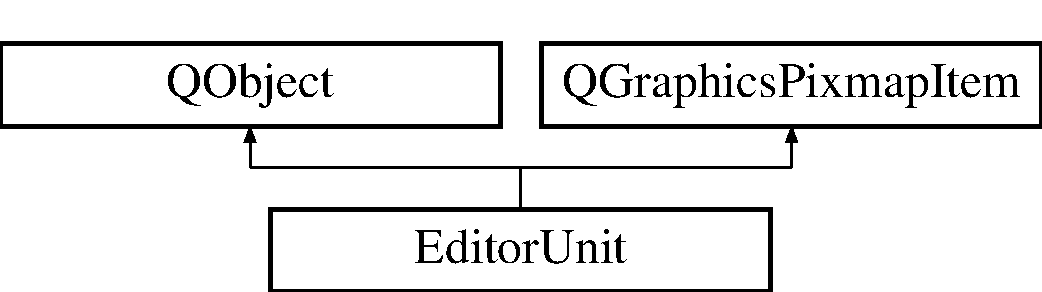
\includegraphics[height=2.000000cm]{class_editor_unit}
\end{center}
\end{figure}
\subsection*{Signals}
\begin{DoxyCompactItemize}
\item 
\hypertarget{class_editor_unit_af4123d742666cb6965f5ea1059ae8631}{}void \hyperlink{class_editor_unit_af4123d742666cb6965f5ea1059ae8631}{unit\+Moved} ()\label{class_editor_unit_af4123d742666cb6965f5ea1059ae8631}

\begin{DoxyCompactList}\small\item\em Signal émit quand le pion est déplacé. \end{DoxyCompactList}\end{DoxyCompactItemize}
\subsection*{Public Member Functions}
\begin{DoxyCompactItemize}
\item 
\hyperlink{class_editor_unit_a3e61a5acc86cfe38923885cd3b16def7}{Editor\+Unit} (Q\+Graphics\+Item $\ast$parent=0)
\begin{DoxyCompactList}\small\item\em Constructeur de base d\textquotesingle{}\hyperlink{class_editor_unit}{Editor\+Unit}. \end{DoxyCompactList}\item 
\hyperlink{class_editor_unit_a96e5806d5fdf9e99605b9545cb26d2cd}{Editor\+Unit} (const Q\+Pixmap \&pixmap, Q\+Graphics\+Item $\ast$parent=0)
\begin{DoxyCompactList}\small\item\em Constructeur avec image d\textquotesingle{}\hyperlink{class_editor_unit}{Editor\+Unit}. \end{DoxyCompactList}\end{DoxyCompactItemize}
\subsection*{Protected Member Functions}
\begin{DoxyCompactItemize}
\item 
void \hyperlink{class_editor_unit_a7a275331118836c72fea1f2ad131881a}{mouse\+Release\+Event} (Q\+Graphics\+Scene\+Mouse\+Event $\ast$event)
\begin{DoxyCompactList}\small\item\em Surchage de la fonction d\textquotesingle{}événement de relâchement de la souris. \end{DoxyCompactList}\end{DoxyCompactItemize}


\subsection{Detailed Description}
Petite classe graphique permettant de bouger un pion. 

\begin{DoxyAuthor}{Author}
Valentin D.\+d.\+G. 
\end{DoxyAuthor}
\begin{DoxyVersion}{Version}
1.\+0 
\end{DoxyVersion}


\subsection{Constructor \& Destructor Documentation}
\hypertarget{class_editor_unit_a3e61a5acc86cfe38923885cd3b16def7}{}\index{Editor\+Unit@{Editor\+Unit}!Editor\+Unit@{Editor\+Unit}}
\index{Editor\+Unit@{Editor\+Unit}!Editor\+Unit@{Editor\+Unit}}
\subsubsection[{Editor\+Unit(\+Q\+Graphics\+Item $\ast$parent=0)}]{\setlength{\rightskip}{0pt plus 5cm}Editor\+Unit\+::\+Editor\+Unit (
\begin{DoxyParamCaption}
\item[{Q\+Graphics\+Item $\ast$}]{parent = {\ttfamily 0}}
\end{DoxyParamCaption}
)}\label{class_editor_unit_a3e61a5acc86cfe38923885cd3b16def7}


Constructeur de base d\textquotesingle{}\hyperlink{class_editor_unit}{Editor\+Unit}. 


\begin{DoxyParams}{Parameters}
{\em parent} & Parent de l\textquotesingle{}objet graphique. \\
\hline
\end{DoxyParams}
\hypertarget{class_editor_unit_a96e5806d5fdf9e99605b9545cb26d2cd}{}\index{Editor\+Unit@{Editor\+Unit}!Editor\+Unit@{Editor\+Unit}}
\index{Editor\+Unit@{Editor\+Unit}!Editor\+Unit@{Editor\+Unit}}
\subsubsection[{Editor\+Unit(const Q\+Pixmap \&pixmap, Q\+Graphics\+Item $\ast$parent=0)}]{\setlength{\rightskip}{0pt plus 5cm}Editor\+Unit\+::\+Editor\+Unit (
\begin{DoxyParamCaption}
\item[{const Q\+Pixmap \&}]{pixmap, }
\item[{Q\+Graphics\+Item $\ast$}]{parent = {\ttfamily 0}}
\end{DoxyParamCaption}
)}\label{class_editor_unit_a96e5806d5fdf9e99605b9545cb26d2cd}


Constructeur avec image d\textquotesingle{}\hyperlink{class_editor_unit}{Editor\+Unit}. 


\begin{DoxyParams}{Parameters}
{\em pixmap} & Image à utiliser \\
\hline
{\em parent} & Parent de l\textquotesingle{}objet graphique. \\
\hline
\end{DoxyParams}


\subsection{Member Function Documentation}
\hypertarget{class_editor_unit_a7a275331118836c72fea1f2ad131881a}{}\index{Editor\+Unit@{Editor\+Unit}!mouse\+Release\+Event@{mouse\+Release\+Event}}
\index{mouse\+Release\+Event@{mouse\+Release\+Event}!Editor\+Unit@{Editor\+Unit}}
\subsubsection[{mouse\+Release\+Event(\+Q\+Graphics\+Scene\+Mouse\+Event $\ast$event)}]{\setlength{\rightskip}{0pt plus 5cm}void Editor\+Unit\+::mouse\+Release\+Event (
\begin{DoxyParamCaption}
\item[{Q\+Graphics\+Scene\+Mouse\+Event $\ast$}]{event}
\end{DoxyParamCaption}
)\hspace{0.3cm}{\ttfamily [protected]}}\label{class_editor_unit_a7a275331118836c72fea1f2ad131881a}


Surchage de la fonction d\textquotesingle{}événement de relâchement de la souris. 


\begin{DoxyParams}{Parameters}
{\em event} & Paramètre généré par l\textquotesingle{}événement. \\
\hline
\end{DoxyParams}


The documentation for this class was generated from the following files\+:\begin{DoxyCompactItemize}
\item 
editorunit.\+h\item 
editorunit.\+cpp\end{DoxyCompactItemize}

\hypertarget{class_ghost_timer}{}\section{Ghost\+Timer Class Reference}
\label{class_ghost_timer}\index{Ghost\+Timer@{Ghost\+Timer}}


Classe de Timer pour les modes des fantômes.  




{\ttfamily \#include $<$ghosttimer.\+h$>$}

\subsection*{Public Member Functions}
\begin{DoxyCompactItemize}
\item 
\hyperlink{class_ghost_timer_adebf7cf8bb544e23f6fd8ce7095b8394}{Ghost\+Timer} ()
\begin{DoxyCompactList}\small\item\em Constructeur de base de la classe \hyperlink{class_ghost_timer}{Ghost\+Timer}. \end{DoxyCompactList}\item 
\hyperlink{class_ghost_timer_a363147268fa53ea5e7f9e4b50b8453ef}{Ghost\+Timer} (Q\+Dom\+Element elem)
\begin{DoxyCompactList}\small\item\em Surcharge du constructeur pour utiliser X\+M\+L. \end{DoxyCompactList}\item 
int \hyperlink{class_ghost_timer_adf6ae0f333a95d4fe3e6f8a132a8201d}{current\+Mode} () const 
\begin{DoxyCompactList}\small\item\em Getter. \end{DoxyCompactList}\item 
void \hyperlink{class_ghost_timer_acca62ab4734e961d46965a7d10a886ad}{increase\+Timer} ()
\begin{DoxyCompactList}\small\item\em Augmente la valeur du timer de T\+I\+M\+E\+\_\+\+B\+E\+T\+W\+E\+E\+N\+\_\+\+F\+R\+A\+M\+E\+S mscs. \end{DoxyCompactList}\end{DoxyCompactItemize}


\subsection{Detailed Description}
Classe de Timer pour les modes des fantômes. 

\begin{DoxyAuthor}{Author}
Valentin D.\+d.\+G. 
\end{DoxyAuthor}
\begin{DoxyVersion}{Version}
1.\+0
\end{DoxyVersion}
Cette classe permet de suivre le mode de poursuite des fantômes en fonction du temps écoulé dans la partie.

Il est nécessaire d\textquotesingle{}appeler manuellement la fonction de mise à jour du timer. 

\subsection{Constructor \& Destructor Documentation}
\hypertarget{class_ghost_timer_adebf7cf8bb544e23f6fd8ce7095b8394}{}\index{Ghost\+Timer@{Ghost\+Timer}!Ghost\+Timer@{Ghost\+Timer}}
\index{Ghost\+Timer@{Ghost\+Timer}!Ghost\+Timer@{Ghost\+Timer}}
\subsubsection[{Ghost\+Timer()}]{\setlength{\rightskip}{0pt plus 5cm}Ghost\+Timer\+::\+Ghost\+Timer (
\begin{DoxyParamCaption}
{}
\end{DoxyParamCaption}
)}\label{class_ghost_timer_adebf7cf8bb544e23f6fd8ce7095b8394}


Constructeur de base de la classe \hyperlink{class_ghost_timer}{Ghost\+Timer}. 

Note \+: Cette version du constructeur n\textquotesingle{}est pas destinée à être utilisée en dehors de l\textquotesingle{}initialisation d\textquotesingle{}une classe qui la contient. L\textquotesingle{}objet créé n\textquotesingle{}est pas valide. \hypertarget{class_ghost_timer_a363147268fa53ea5e7f9e4b50b8453ef}{}\index{Ghost\+Timer@{Ghost\+Timer}!Ghost\+Timer@{Ghost\+Timer}}
\index{Ghost\+Timer@{Ghost\+Timer}!Ghost\+Timer@{Ghost\+Timer}}
\subsubsection[{Ghost\+Timer(\+Q\+Dom\+Element elem)}]{\setlength{\rightskip}{0pt plus 5cm}Ghost\+Timer\+::\+Ghost\+Timer (
\begin{DoxyParamCaption}
\item[{Q\+Dom\+Element}]{elem}
\end{DoxyParamCaption}
)}\label{class_ghost_timer_a363147268fa53ea5e7f9e4b50b8453ef}


Surcharge du constructeur pour utiliser X\+M\+L. 


\begin{DoxyParams}{Parameters}
{\em elem} & Données X\+M\+L à charger lors de la contruction de l\textquotesingle{}objet.\\
\hline
\end{DoxyParams}
L\textquotesingle{}élément X\+M\+L doit ressembler au template suivant \+:
\begin{DoxyItemize}
\item $<$\hyperlink{class_ghost_timer}{Ghost\+Timer}$>$
\begin{DoxyItemize}
\item $<$Step time=\char`\"{}7\char`\"{} mode=\char`\"{}0\char`\"{}/$>$ // Mode Scatter (0) pendant 7 secondes.
\item $<$Step time=\char`\"{}20\char`\"{} mode=\char`\"{}1\char`\"{}/$>$ // Puis Chase(1) pendant 20 secondes.
\item $<$Step time=\char`\"{}7\char`\"{} mode=\char`\"{}0\char`\"{}/$>$ // Puis Scatter (0) jusqu\textquotesingle{}à la fin (time ignoré).
\end{DoxyItemize}
\item $<$/\+Ghost\+Timer$>$ 
\end{DoxyItemize}

\subsection{Member Function Documentation}
\hypertarget{class_ghost_timer_adf6ae0f333a95d4fe3e6f8a132a8201d}{}\index{Ghost\+Timer@{Ghost\+Timer}!current\+Mode@{current\+Mode}}
\index{current\+Mode@{current\+Mode}!Ghost\+Timer@{Ghost\+Timer}}
\subsubsection[{current\+Mode() const }]{\setlength{\rightskip}{0pt plus 5cm}int Ghost\+Timer\+::current\+Mode (
\begin{DoxyParamCaption}
{}
\end{DoxyParamCaption}
) const}\label{class_ghost_timer_adf6ae0f333a95d4fe3e6f8a132a8201d}


Getter. 

\begin{DoxyReturn}{Returns}
Mode de poursuite actuel du timer. 
\end{DoxyReturn}
\hypertarget{class_ghost_timer_acca62ab4734e961d46965a7d10a886ad}{}\index{Ghost\+Timer@{Ghost\+Timer}!increase\+Timer@{increase\+Timer}}
\index{increase\+Timer@{increase\+Timer}!Ghost\+Timer@{Ghost\+Timer}}
\subsubsection[{increase\+Timer()}]{\setlength{\rightskip}{0pt plus 5cm}void Ghost\+Timer\+::increase\+Timer (
\begin{DoxyParamCaption}
{}
\end{DoxyParamCaption}
)}\label{class_ghost_timer_acca62ab4734e961d46965a7d10a886ad}


Augmente la valeur du timer de T\+I\+M\+E\+\_\+\+B\+E\+T\+W\+E\+E\+N\+\_\+\+F\+R\+A\+M\+E\+S mscs. 

Si la valeur excède la prochaine limite de temps, le timer passe au prochain mode et réinitialise sa valeur de temps. 

The documentation for this class was generated from the following files\+:\begin{DoxyCompactItemize}
\item 
ghosttimer.\+h\item 
ghosttimer.\+cpp\end{DoxyCompactItemize}

\hypertarget{class_main_window}{}\section{Main\+Window Class Reference}
\label{class_main_window}\index{Main\+Window@{Main\+Window}}


Classe de fenêtre principale.  




{\ttfamily \#include $<$mainwindow.\+h$>$}

Inheritance diagram for Main\+Window\+:\begin{figure}[H]
\begin{center}
\leavevmode
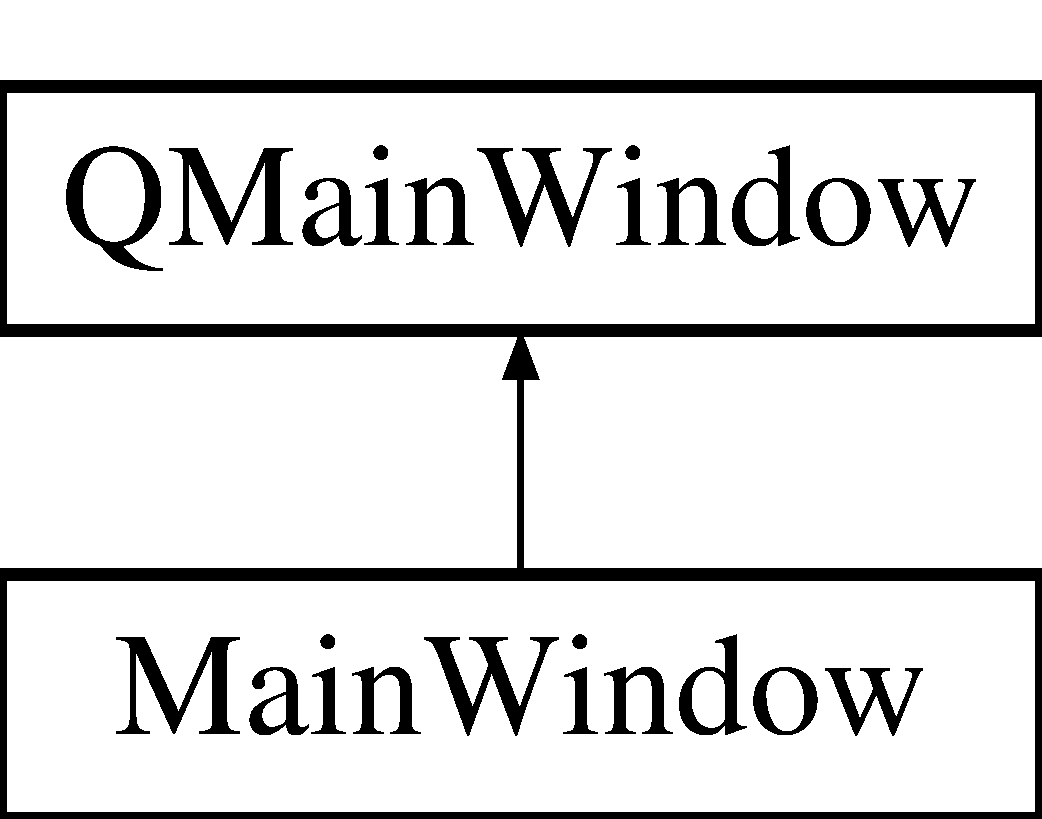
\includegraphics[height=2.000000cm]{class_main_window}
\end{center}
\end{figure}
\subsection*{Public Member Functions}
\begin{DoxyCompactItemize}
\item 
\hyperlink{class_main_window_a8b244be8b7b7db1b08de2a2acb9409db}{Main\+Window} (Q\+Widget $\ast$parent=0)
\begin{DoxyCompactList}\small\item\em Constructeur de base de la classe \hyperlink{class_main_window}{Main\+Window}. \end{DoxyCompactList}\item 
\hypertarget{class_main_window_ae98d00a93bc118200eeef9f9bba1dba7}{}\hyperlink{class_main_window_ae98d00a93bc118200eeef9f9bba1dba7}{$\sim$\+Main\+Window} ()\label{class_main_window_ae98d00a93bc118200eeef9f9bba1dba7}

\begin{DoxyCompactList}\small\item\em Destructeur de la classe \hyperlink{class_main_window}{Main\+Window}. \end{DoxyCompactList}\end{DoxyCompactItemize}


\subsection{Detailed Description}
Classe de fenêtre principale. 

\begin{DoxyAuthor}{Author}
Valentin D.\+d.\+G. 
\end{DoxyAuthor}
\begin{DoxyVersion}{Version}
1.\+0
\end{DoxyVersion}
Cette classe intialise les objets principaux du jeu.


\begin{DoxyItemize}
\item Note \+: Dans l\textquotesingle{}avenir, elle permettra éventuellement un menu dirigeant vers l\textquotesingle{}éditeur de niveaux. 
\end{DoxyItemize}

\subsection{Constructor \& Destructor Documentation}
\hypertarget{class_main_window_a8b244be8b7b7db1b08de2a2acb9409db}{}\index{Main\+Window@{Main\+Window}!Main\+Window@{Main\+Window}}
\index{Main\+Window@{Main\+Window}!Main\+Window@{Main\+Window}}
\subsubsection[{Main\+Window(\+Q\+Widget $\ast$parent=0)}]{\setlength{\rightskip}{0pt plus 5cm}Main\+Window\+::\+Main\+Window (
\begin{DoxyParamCaption}
\item[{Q\+Widget $\ast$}]{parent = {\ttfamily 0}}
\end{DoxyParamCaption}
)\hspace{0.3cm}{\ttfamily [explicit]}}\label{class_main_window_a8b244be8b7b7db1b08de2a2acb9409db}


Constructeur de base de la classe \hyperlink{class_main_window}{Main\+Window}. 


\begin{DoxyParams}{Parameters}
{\em parent} & Parent de la fenêtre (devrait être nul). \\
\hline
\end{DoxyParams}


The documentation for this class was generated from the following files\+:\begin{DoxyCompactItemize}
\item 
mainwindow.\+h\item 
mainwindow.\+cpp\end{DoxyCompactItemize}

\hypertarget{class_map}{}\section{Map Class Reference}
\label{class_map}\index{Map@{Map}}


Objet graphique détectant les clics souris et générant des signaux.  




{\ttfamily \#include $<$map.\+h$>$}

Inheritance diagram for Map\+:\begin{figure}[H]
\begin{center}
\leavevmode
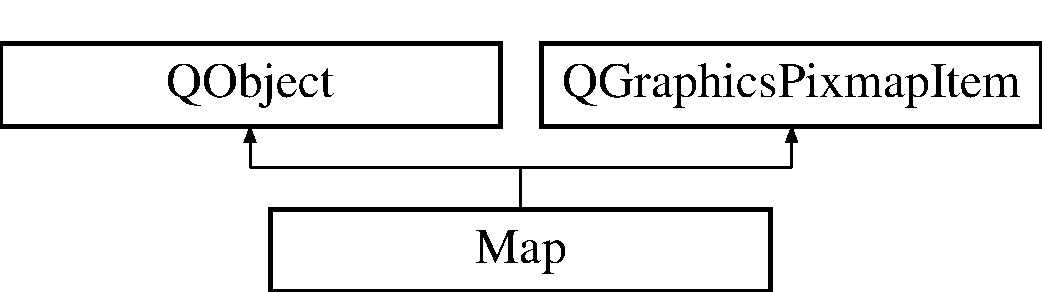
\includegraphics[height=2.000000cm]{class_map}
\end{center}
\end{figure}
\subsection*{Signals}
\begin{DoxyCompactItemize}
\item 
void \hyperlink{class_map_a43f303132cbb28cf95244e40aa030dbe}{map\+Clicked} (Q\+Graphics\+Scene\+Mouse\+Event $\ast$event)
\begin{DoxyCompactList}\small\item\em Signal émit lorsque l\textquotesingle{}on clic sur l\textquotesingle{}objet graphique. \end{DoxyCompactList}\end{DoxyCompactItemize}
\subsection*{Public Member Functions}
\begin{DoxyCompactItemize}
\item 
\hypertarget{class_map_a0f5ad0fd4563497b4214038cbca8b582}{}\hyperlink{class_map_a0f5ad0fd4563497b4214038cbca8b582}{Map} ()\label{class_map_a0f5ad0fd4563497b4214038cbca8b582}

\begin{DoxyCompactList}\small\item\em Constructeur de base de \hyperlink{class_map}{Map}. \end{DoxyCompactList}\end{DoxyCompactItemize}
\subsection*{Protected Member Functions}
\begin{DoxyCompactItemize}
\item 
void \hyperlink{class_map_a647f0a0188e709b564a5127ca8d71d67}{mouse\+Press\+Event} (Q\+Graphics\+Scene\+Mouse\+Event $\ast$event)
\begin{DoxyCompactList}\small\item\em Surchage de la fonction d\textquotesingle{}événement d\textquotesingle{}appui de la souris. \end{DoxyCompactList}\end{DoxyCompactItemize}


\subsection{Detailed Description}
Objet graphique détectant les clics souris et générant des signaux. 

\begin{DoxyAuthor}{Author}
Valentin D.\+d.\+G. 
\end{DoxyAuthor}
\begin{DoxyVersion}{Version}
1.\+0 
\end{DoxyVersion}


\subsection{Member Function Documentation}
\hypertarget{class_map_a43f303132cbb28cf95244e40aa030dbe}{}\index{Map@{Map}!map\+Clicked@{map\+Clicked}}
\index{map\+Clicked@{map\+Clicked}!Map@{Map}}
\subsubsection[{map\+Clicked}]{\setlength{\rightskip}{0pt plus 5cm}void Map\+::map\+Clicked (
\begin{DoxyParamCaption}
\item[{Q\+Graphics\+Scene\+Mouse\+Event $\ast$}]{event}
\end{DoxyParamCaption}
)\hspace{0.3cm}{\ttfamily [signal]}}\label{class_map_a43f303132cbb28cf95244e40aa030dbe}


Signal émit lorsque l\textquotesingle{}on clic sur l\textquotesingle{}objet graphique. 


\begin{DoxyParams}{Parameters}
{\em event} & Paramètre généré par l\textquotesingle{}événement. \\
\hline
\end{DoxyParams}
\hypertarget{class_map_a647f0a0188e709b564a5127ca8d71d67}{}\index{Map@{Map}!mouse\+Press\+Event@{mouse\+Press\+Event}}
\index{mouse\+Press\+Event@{mouse\+Press\+Event}!Map@{Map}}
\subsubsection[{mouse\+Press\+Event(\+Q\+Graphics\+Scene\+Mouse\+Event $\ast$event)}]{\setlength{\rightskip}{0pt plus 5cm}void Map\+::mouse\+Press\+Event (
\begin{DoxyParamCaption}
\item[{Q\+Graphics\+Scene\+Mouse\+Event $\ast$}]{event}
\end{DoxyParamCaption}
)\hspace{0.3cm}{\ttfamily [protected]}}\label{class_map_a647f0a0188e709b564a5127ca8d71d67}


Surchage de la fonction d\textquotesingle{}événement d\textquotesingle{}appui de la souris. 


\begin{DoxyParams}{Parameters}
{\em event} & Paramètre généré par l\textquotesingle{}événement. \\
\hline
\end{DoxyParams}


The documentation for this class was generated from the following files\+:\begin{DoxyCompactItemize}
\item 
map.\+h\item 
map.\+cpp\end{DoxyCompactItemize}

\hypertarget{class_new_ghost_mode_dialog}{}\section{New\+Ghost\+Mode\+Dialog Class Reference}
\label{class_new_ghost_mode_dialog}\index{New\+Ghost\+Mode\+Dialog@{New\+Ghost\+Mode\+Dialog}}


Classe graphique de fenêtre pour l\textquotesingle{}ajout d\textquotesingle{}un nouveau mode de poursuite.  




{\ttfamily \#include $<$newghostmodedialog.\+h$>$}

Inheritance diagram for New\+Ghost\+Mode\+Dialog\+:\begin{figure}[H]
\begin{center}
\leavevmode
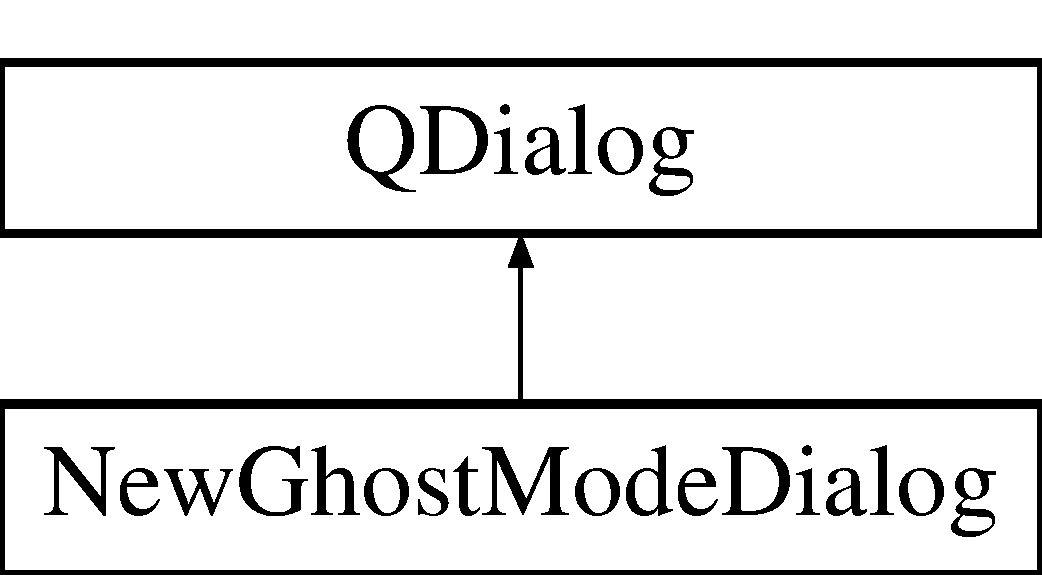
\includegraphics[height=2.000000cm]{class_new_ghost_mode_dialog}
\end{center}
\end{figure}
\subsection*{Public Member Functions}
\begin{DoxyCompactItemize}
\item 
\hyperlink{class_new_ghost_mode_dialog_ac38be81a34c8e2a6c9582a29beeb1acd}{New\+Ghost\+Mode\+Dialog} (Q\+Widget $\ast$parent=0)
\begin{DoxyCompactList}\small\item\em Constructeur de base de \hyperlink{class_new_ghost_mode_dialog}{New\+Ghost\+Mode\+Dialog}. \end{DoxyCompactList}\item 
\hypertarget{class_new_ghost_mode_dialog_a4b7ed89ce68bb09cfaa5aebb1f484130}{}\hyperlink{class_new_ghost_mode_dialog_a4b7ed89ce68bb09cfaa5aebb1f484130}{$\sim$\+New\+Ghost\+Mode\+Dialog} ()\label{class_new_ghost_mode_dialog_a4b7ed89ce68bb09cfaa5aebb1f484130}

\begin{DoxyCompactList}\small\item\em Destructeur de \hyperlink{class_new_ghost_mode_dialog}{New\+Ghost\+Mode\+Dialog}. \end{DoxyCompactList}\item 
int \hyperlink{class_new_ghost_mode_dialog_aae6742233da69550c9ae1e1916ac4591}{duration} () const 
\begin{DoxyCompactList}\small\item\em Getter. \end{DoxyCompactList}\item 
int \hyperlink{class_new_ghost_mode_dialog_a73406f3e476866566fb17d8ca319ecda}{mode} () const 
\begin{DoxyCompactList}\small\item\em Getter. \end{DoxyCompactList}\end{DoxyCompactItemize}


\subsection{Detailed Description}
Classe graphique de fenêtre pour l\textquotesingle{}ajout d\textquotesingle{}un nouveau mode de poursuite. 

\begin{DoxyAuthor}{Author}
Valentin D.\+d.\+G. 
\end{DoxyAuthor}
\begin{DoxyVersion}{Version}
1.\+0 
\end{DoxyVersion}


\subsection{Constructor \& Destructor Documentation}
\hypertarget{class_new_ghost_mode_dialog_ac38be81a34c8e2a6c9582a29beeb1acd}{}\index{New\+Ghost\+Mode\+Dialog@{New\+Ghost\+Mode\+Dialog}!New\+Ghost\+Mode\+Dialog@{New\+Ghost\+Mode\+Dialog}}
\index{New\+Ghost\+Mode\+Dialog@{New\+Ghost\+Mode\+Dialog}!New\+Ghost\+Mode\+Dialog@{New\+Ghost\+Mode\+Dialog}}
\subsubsection[{New\+Ghost\+Mode\+Dialog(\+Q\+Widget $\ast$parent=0)}]{\setlength{\rightskip}{0pt plus 5cm}New\+Ghost\+Mode\+Dialog\+::\+New\+Ghost\+Mode\+Dialog (
\begin{DoxyParamCaption}
\item[{Q\+Widget $\ast$}]{parent = {\ttfamily 0}}
\end{DoxyParamCaption}
)\hspace{0.3cm}{\ttfamily [explicit]}}\label{class_new_ghost_mode_dialog_ac38be81a34c8e2a6c9582a29beeb1acd}


Constructeur de base de \hyperlink{class_new_ghost_mode_dialog}{New\+Ghost\+Mode\+Dialog}. 


\begin{DoxyParams}{Parameters}
{\em parent} & Parent de la fenêtre. \\
\hline
\end{DoxyParams}


\subsection{Member Function Documentation}
\hypertarget{class_new_ghost_mode_dialog_aae6742233da69550c9ae1e1916ac4591}{}\index{New\+Ghost\+Mode\+Dialog@{New\+Ghost\+Mode\+Dialog}!duration@{duration}}
\index{duration@{duration}!New\+Ghost\+Mode\+Dialog@{New\+Ghost\+Mode\+Dialog}}
\subsubsection[{duration() const }]{\setlength{\rightskip}{0pt plus 5cm}int New\+Ghost\+Mode\+Dialog\+::duration (
\begin{DoxyParamCaption}
{}
\end{DoxyParamCaption}
) const}\label{class_new_ghost_mode_dialog_aae6742233da69550c9ae1e1916ac4591}


Getter. 

\begin{DoxyReturn}{Returns}
Durée où le mode est actif. 
\end{DoxyReturn}
\hypertarget{class_new_ghost_mode_dialog_a73406f3e476866566fb17d8ca319ecda}{}\index{New\+Ghost\+Mode\+Dialog@{New\+Ghost\+Mode\+Dialog}!mode@{mode}}
\index{mode@{mode}!New\+Ghost\+Mode\+Dialog@{New\+Ghost\+Mode\+Dialog}}
\subsubsection[{mode() const }]{\setlength{\rightskip}{0pt plus 5cm}int New\+Ghost\+Mode\+Dialog\+::mode (
\begin{DoxyParamCaption}
{}
\end{DoxyParamCaption}
) const}\label{class_new_ghost_mode_dialog_a73406f3e476866566fb17d8ca319ecda}


Getter. 

\begin{DoxyReturn}{Returns}
Type de mode actif. 
\end{DoxyReturn}


The documentation for this class was generated from the following files\+:\begin{DoxyCompactItemize}
\item 
newghostmodedialog.\+h\item 
newghostmodedialog.\+cpp\end{DoxyCompactItemize}

\hypertarget{class_new_level_dialog}{}\section{New\+Level\+Dialog Class Reference}
\label{class_new_level_dialog}\index{New\+Level\+Dialog@{New\+Level\+Dialog}}


Classe graphique de fenêtre pour l\textquotesingle{}ajout d\textquotesingle{}un nouveau niveaau.  




{\ttfamily \#include $<$newleveldialog.\+h$>$}

Inheritance diagram for New\+Level\+Dialog\+:\begin{figure}[H]
\begin{center}
\leavevmode
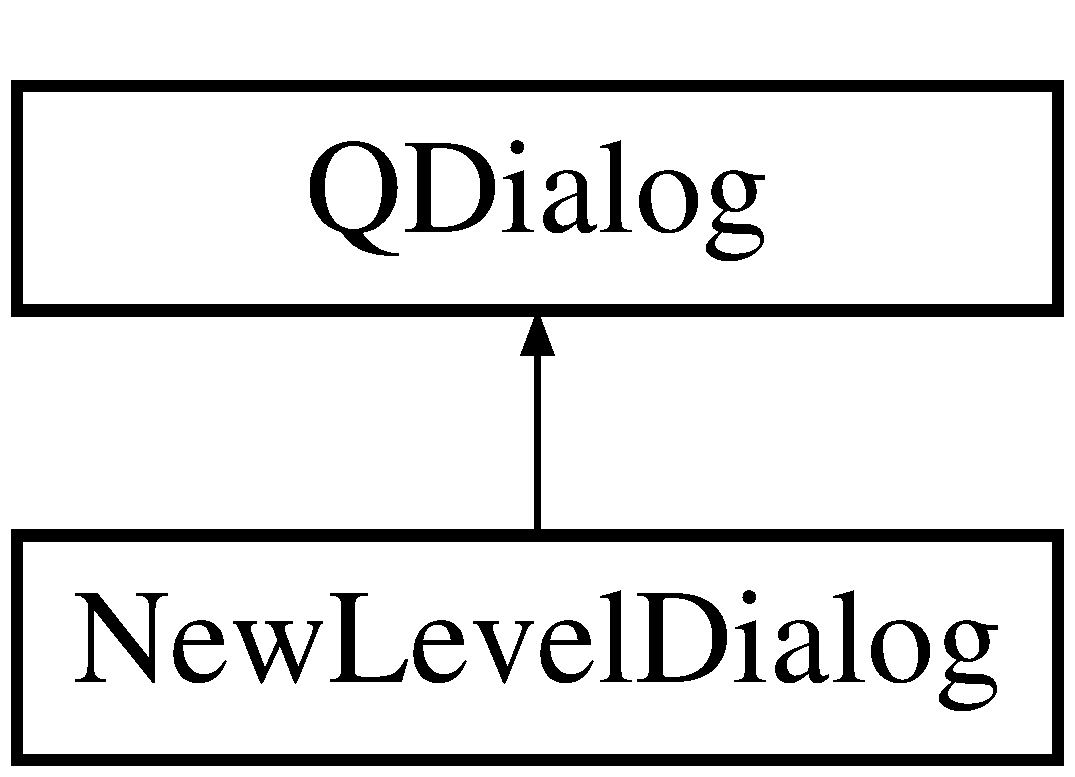
\includegraphics[height=2.000000cm]{class_new_level_dialog}
\end{center}
\end{figure}
\subsection*{Public Member Functions}
\begin{DoxyCompactItemize}
\item 
\hyperlink{class_new_level_dialog_ad177ac13535e71bc671a0c04f0464854}{New\+Level\+Dialog} (bool previous\+Grid\+Available, Q\+Widget $\ast$parent=0)
\begin{DoxyCompactList}\small\item\em Constructeur de base de \hyperlink{class_new_level_dialog}{New\+Level\+Dialog}. \end{DoxyCompactList}\item 
\hyperlink{class_new_level_dialog_abb85c197f87a69f2faae637bb5247897}{$\sim$\+New\+Level\+Dialog} ()
\item 
Q\+Size \hyperlink{class_new_level_dialog_a5ca7d9a32d6afb209dc63c12836de28d}{grid\+Size} () const 
\begin{DoxyCompactList}\small\item\em Getter. \end{DoxyCompactList}\item 
int \hyperlink{class_new_level_dialog_a719c671d7b868e298b07471afba279ea}{tile\+Count\+Width} () const 
\begin{DoxyCompactList}\small\item\em Getter. \end{DoxyCompactList}\item 
int \hyperlink{class_new_level_dialog_a0144b7e9d62d1d3e51f59801e7e20f3e}{tile\+Count\+Height} () const 
\begin{DoxyCompactList}\small\item\em Getter. \end{DoxyCompactList}\item 
int \hyperlink{class_new_level_dialog_a1f7bb6871337ead5bdd8bdbfca292aea}{tile\+Size} () const 
\begin{DoxyCompactList}\small\item\em Getter. \end{DoxyCompactList}\item 
Q\+String \hyperlink{class_new_level_dialog_ae155692ae9fa604ac0955d9d2882afd0}{level\+Name} () const 
\begin{DoxyCompactList}\small\item\em Getter. \end{DoxyCompactList}\item 
bool \hyperlink{class_new_level_dialog_a35dc3afda2c0d098e982daa400fc0876}{use\+Previous\+Grid} () const 
\begin{DoxyCompactList}\small\item\em Getter. \end{DoxyCompactList}\end{DoxyCompactItemize}


\subsection{Detailed Description}
Classe graphique de fenêtre pour l\textquotesingle{}ajout d\textquotesingle{}un nouveau niveaau. 

\begin{DoxyAuthor}{Author}
Valentin D.\+d.\+G. 
\end{DoxyAuthor}
\begin{DoxyVersion}{Version}
1.\+0 
\end{DoxyVersion}


\subsection{Constructor \& Destructor Documentation}
\hypertarget{class_new_level_dialog_ad177ac13535e71bc671a0c04f0464854}{}\index{New\+Level\+Dialog@{New\+Level\+Dialog}!New\+Level\+Dialog@{New\+Level\+Dialog}}
\index{New\+Level\+Dialog@{New\+Level\+Dialog}!New\+Level\+Dialog@{New\+Level\+Dialog}}
\subsubsection[{New\+Level\+Dialog(bool previous\+Grid\+Available, Q\+Widget $\ast$parent=0)}]{\setlength{\rightskip}{0pt plus 5cm}New\+Level\+Dialog\+::\+New\+Level\+Dialog (
\begin{DoxyParamCaption}
\item[{bool}]{previous\+Grid\+Available, }
\item[{Q\+Widget $\ast$}]{parent = {\ttfamily 0}}
\end{DoxyParamCaption}
)\hspace{0.3cm}{\ttfamily [explicit]}}\label{class_new_level_dialog_ad177ac13535e71bc671a0c04f0464854}


Constructeur de base de \hyperlink{class_new_level_dialog}{New\+Level\+Dialog}. 


\begin{DoxyParams}{Parameters}
{\em previous\+Grid\+Available} & Si vrai, active les champs de récupération de la grille précédente. \\
\hline
{\em parent} & Parent de la fenêtre. \\
\hline
\end{DoxyParams}
\hypertarget{class_new_level_dialog_abb85c197f87a69f2faae637bb5247897}{}\index{New\+Level\+Dialog@{New\+Level\+Dialog}!````~New\+Level\+Dialog@{$\sim$\+New\+Level\+Dialog}}
\index{````~New\+Level\+Dialog@{$\sim$\+New\+Level\+Dialog}!New\+Level\+Dialog@{New\+Level\+Dialog}}
\subsubsection[{$\sim$\+New\+Level\+Dialog()}]{\setlength{\rightskip}{0pt plus 5cm}New\+Level\+Dialog\+::$\sim$\+New\+Level\+Dialog (
\begin{DoxyParamCaption}
{}
\end{DoxyParamCaption}
)}\label{class_new_level_dialog_abb85c197f87a69f2faae637bb5247897}
Destructeur de \hyperlink{class_new_level_dialog}{New\+Level\+Dialog} 

\subsection{Member Function Documentation}
\hypertarget{class_new_level_dialog_a5ca7d9a32d6afb209dc63c12836de28d}{}\index{New\+Level\+Dialog@{New\+Level\+Dialog}!grid\+Size@{grid\+Size}}
\index{grid\+Size@{grid\+Size}!New\+Level\+Dialog@{New\+Level\+Dialog}}
\subsubsection[{grid\+Size() const }]{\setlength{\rightskip}{0pt plus 5cm}Q\+Size New\+Level\+Dialog\+::grid\+Size (
\begin{DoxyParamCaption}
{}
\end{DoxyParamCaption}
) const}\label{class_new_level_dialog_a5ca7d9a32d6afb209dc63c12836de28d}


Getter. 

\begin{DoxyReturn}{Returns}
Taille de la grille (nombre de case). 
\end{DoxyReturn}
\hypertarget{class_new_level_dialog_ae155692ae9fa604ac0955d9d2882afd0}{}\index{New\+Level\+Dialog@{New\+Level\+Dialog}!level\+Name@{level\+Name}}
\index{level\+Name@{level\+Name}!New\+Level\+Dialog@{New\+Level\+Dialog}}
\subsubsection[{level\+Name() const }]{\setlength{\rightskip}{0pt plus 5cm}Q\+String New\+Level\+Dialog\+::level\+Name (
\begin{DoxyParamCaption}
{}
\end{DoxyParamCaption}
) const}\label{class_new_level_dialog_ae155692ae9fa604ac0955d9d2882afd0}


Getter. 

\begin{DoxyReturn}{Returns}
Nom du niveau. 
\end{DoxyReturn}
\hypertarget{class_new_level_dialog_a0144b7e9d62d1d3e51f59801e7e20f3e}{}\index{New\+Level\+Dialog@{New\+Level\+Dialog}!tile\+Count\+Height@{tile\+Count\+Height}}
\index{tile\+Count\+Height@{tile\+Count\+Height}!New\+Level\+Dialog@{New\+Level\+Dialog}}
\subsubsection[{tile\+Count\+Height() const }]{\setlength{\rightskip}{0pt plus 5cm}int New\+Level\+Dialog\+::tile\+Count\+Height (
\begin{DoxyParamCaption}
{}
\end{DoxyParamCaption}
) const}\label{class_new_level_dialog_a0144b7e9d62d1d3e51f59801e7e20f3e}


Getter. 

\begin{DoxyReturn}{Returns}
Nombre de case en hauteur. 
\end{DoxyReturn}
\hypertarget{class_new_level_dialog_a719c671d7b868e298b07471afba279ea}{}\index{New\+Level\+Dialog@{New\+Level\+Dialog}!tile\+Count\+Width@{tile\+Count\+Width}}
\index{tile\+Count\+Width@{tile\+Count\+Width}!New\+Level\+Dialog@{New\+Level\+Dialog}}
\subsubsection[{tile\+Count\+Width() const }]{\setlength{\rightskip}{0pt plus 5cm}int New\+Level\+Dialog\+::tile\+Count\+Width (
\begin{DoxyParamCaption}
{}
\end{DoxyParamCaption}
) const}\label{class_new_level_dialog_a719c671d7b868e298b07471afba279ea}


Getter. 

\begin{DoxyReturn}{Returns}
Nombre de case en largeur. 
\end{DoxyReturn}
\hypertarget{class_new_level_dialog_a1f7bb6871337ead5bdd8bdbfca292aea}{}\index{New\+Level\+Dialog@{New\+Level\+Dialog}!tile\+Size@{tile\+Size}}
\index{tile\+Size@{tile\+Size}!New\+Level\+Dialog@{New\+Level\+Dialog}}
\subsubsection[{tile\+Size() const }]{\setlength{\rightskip}{0pt plus 5cm}int New\+Level\+Dialog\+::tile\+Size (
\begin{DoxyParamCaption}
{}
\end{DoxyParamCaption}
) const}\label{class_new_level_dialog_a1f7bb6871337ead5bdd8bdbfca292aea}


Getter. 

\begin{DoxyReturn}{Returns}
Taille d\textquotesingle{}une case (en pixels). 
\end{DoxyReturn}
\hypertarget{class_new_level_dialog_a35dc3afda2c0d098e982daa400fc0876}{}\index{New\+Level\+Dialog@{New\+Level\+Dialog}!use\+Previous\+Grid@{use\+Previous\+Grid}}
\index{use\+Previous\+Grid@{use\+Previous\+Grid}!New\+Level\+Dialog@{New\+Level\+Dialog}}
\subsubsection[{use\+Previous\+Grid() const }]{\setlength{\rightskip}{0pt plus 5cm}bool New\+Level\+Dialog\+::use\+Previous\+Grid (
\begin{DoxyParamCaption}
{}
\end{DoxyParamCaption}
) const}\label{class_new_level_dialog_a35dc3afda2c0d098e982daa400fc0876}


Getter. 

\begin{DoxyReturn}{Returns}
Vrai si l\textquotesingle{}option \char`\"{}\+Utiliser grille précédente\char`\"{} a été cochée, Faux sinon. 
\end{DoxyReturn}


The documentation for this class was generated from the following files\+:\begin{DoxyCompactItemize}
\item 
newleveldialog.\+h\item 
newleveldialog.\+cpp\end{DoxyCompactItemize}

\hypertarget{class_texture_handler}{}\section{Texture\+Handler Class Reference}
\label{class_texture_handler}\index{Texture\+Handler@{Texture\+Handler}}


Gestionnaire de textures.  




{\ttfamily \#include $<$texturehandler.\+h$>$}

\subsection*{Public Member Functions}
\begin{DoxyCompactItemize}
\item 
\hyperlink{class_texture_handler_a9056de3d9a44b2e696c8e8b39462dd46}{Texture\+Handler} ()
\begin{DoxyCompactList}\small\item\em Constructeur de base de \hyperlink{class_texture_handler}{Texture\+Handler}. \end{DoxyCompactList}\item 
void \hyperlink{class_texture_handler_a67bc892bd24dfd85bc1eb3af78b8ca40}{add\+Texture} (Q\+String complete\+Filename)
\begin{DoxyCompactList}\small\item\em Ajoute une texture via le chemin du fichier. \end{DoxyCompactList}\item 
Q\+Pixmap \hyperlink{class_texture_handler_a608d66882a46775d1ce498895cf3679b}{texture\+At} (int index) const 
\begin{DoxyCompactList}\small\item\em Getter. \end{DoxyCompactList}\item 
Q\+String \hyperlink{class_texture_handler_a0cdb224be8b1980733698f41b856a55c}{filename\+At} (int index) const 
\begin{DoxyCompactList}\small\item\em Getter. \end{DoxyCompactList}\item 
Q\+String \hyperlink{class_texture_handler_aa6d8737d949687142ffff1e163a15b4f}{texture\+Name\+At} (int index) const 
\begin{DoxyCompactList}\small\item\em Getter. \end{DoxyCompactList}\item 
bool \hyperlink{class_texture_handler_a28014e2b89614335ec2131cdfb94c0be}{contains} (Q\+String filename) const 
\begin{DoxyCompactList}\small\item\em Vérifie si le gestionnaire connait déjà la texture donnée. \end{DoxyCompactList}\item 
int \hyperlink{class_texture_handler_a4753c03df1e7718542557000c04988b1}{index\+Of\+Texture\+Name} (Q\+String texture\+Name) const 
\begin{DoxyCompactList}\small\item\em Récupère l\textquotesingle{}index de la texture dans le gestionnaire. \end{DoxyCompactList}\item 
int \hyperlink{class_texture_handler_aa3fe3f090ff350d2357b4b6fdb570eb7}{count} () const 
\begin{DoxyCompactList}\small\item\em Getter. \end{DoxyCompactList}\item 
int \hyperlink{class_texture_handler_a57242ce71321d2d3376f621486bd432c}{tiles\+Size} () const 
\begin{DoxyCompactList}\small\item\em Getter. \end{DoxyCompactList}\item 
void \hyperlink{class_texture_handler_aecf95d09a430bbc7b92f0a2189b9ff7d}{set\+Tiles\+Size} (int \hyperlink{class_texture_handler_a57242ce71321d2d3376f621486bd432c}{tiles\+Size})
\begin{DoxyCompactList}\small\item\em Setter. \end{DoxyCompactList}\end{DoxyCompactItemize}


\subsection{Detailed Description}
Gestionnaire de textures. 

\begin{DoxyAuthor}{Author}
Valentin D.\+d.\+G. 
\end{DoxyAuthor}
\begin{DoxyVersion}{Version}
1.\+0
\end{DoxyVersion}
Ce gestionnaire de textures permet de faire le lien entre le nom complet d\textquotesingle{}un fichier, son nom en court et son index dans le gestionnaire. Le gestionnaire par défaut modifie la taille des textures. 

\subsection{Constructor \& Destructor Documentation}
\hypertarget{class_texture_handler_a9056de3d9a44b2e696c8e8b39462dd46}{}\index{Texture\+Handler@{Texture\+Handler}!Texture\+Handler@{Texture\+Handler}}
\index{Texture\+Handler@{Texture\+Handler}!Texture\+Handler@{Texture\+Handler}}
\subsubsection[{Texture\+Handler()}]{\setlength{\rightskip}{0pt plus 5cm}Texture\+Handler\+::\+Texture\+Handler (
\begin{DoxyParamCaption}
{}
\end{DoxyParamCaption}
)}\label{class_texture_handler_a9056de3d9a44b2e696c8e8b39462dd46}


Constructeur de base de \hyperlink{class_texture_handler}{Texture\+Handler}. 

Crée un gestionnaire totalement vide. 

\subsection{Member Function Documentation}
\hypertarget{class_texture_handler_a67bc892bd24dfd85bc1eb3af78b8ca40}{}\index{Texture\+Handler@{Texture\+Handler}!add\+Texture@{add\+Texture}}
\index{add\+Texture@{add\+Texture}!Texture\+Handler@{Texture\+Handler}}
\subsubsection[{add\+Texture(\+Q\+String complete\+Filename)}]{\setlength{\rightskip}{0pt plus 5cm}void Texture\+Handler\+::add\+Texture (
\begin{DoxyParamCaption}
\item[{Q\+String}]{complete\+Filename}
\end{DoxyParamCaption}
)}\label{class_texture_handler_a67bc892bd24dfd85bc1eb3af78b8ca40}


Ajoute une texture via le chemin du fichier. 


\begin{DoxyParams}{Parameters}
{\em complete\+Filename} & Chemin complet vers la texture ajoutée. \\
\hline
\end{DoxyParams}
\hypertarget{class_texture_handler_a28014e2b89614335ec2131cdfb94c0be}{}\index{Texture\+Handler@{Texture\+Handler}!contains@{contains}}
\index{contains@{contains}!Texture\+Handler@{Texture\+Handler}}
\subsubsection[{contains(\+Q\+String filename) const }]{\setlength{\rightskip}{0pt plus 5cm}bool Texture\+Handler\+::contains (
\begin{DoxyParamCaption}
\item[{Q\+String}]{filename}
\end{DoxyParamCaption}
) const}\label{class_texture_handler_a28014e2b89614335ec2131cdfb94c0be}


Vérifie si le gestionnaire connait déjà la texture donnée. 


\begin{DoxyParams}{Parameters}
{\em filename} & Chemin complet vers la texture. \\
\hline
\end{DoxyParams}
\begin{DoxyReturn}{Returns}
Vrai si le gestionnaire contient la texture, sinon Faux. 
\end{DoxyReturn}
\hypertarget{class_texture_handler_aa3fe3f090ff350d2357b4b6fdb570eb7}{}\index{Texture\+Handler@{Texture\+Handler}!count@{count}}
\index{count@{count}!Texture\+Handler@{Texture\+Handler}}
\subsubsection[{count() const }]{\setlength{\rightskip}{0pt plus 5cm}int Texture\+Handler\+::count (
\begin{DoxyParamCaption}
{}
\end{DoxyParamCaption}
) const}\label{class_texture_handler_aa3fe3f090ff350d2357b4b6fdb570eb7}


Getter. 

\begin{DoxyReturn}{Returns}
Nombre de textures différentes stockées. 
\end{DoxyReturn}
\hypertarget{class_texture_handler_a0cdb224be8b1980733698f41b856a55c}{}\index{Texture\+Handler@{Texture\+Handler}!filename\+At@{filename\+At}}
\index{filename\+At@{filename\+At}!Texture\+Handler@{Texture\+Handler}}
\subsubsection[{filename\+At(int index) const }]{\setlength{\rightskip}{0pt plus 5cm}Q\+String Texture\+Handler\+::filename\+At (
\begin{DoxyParamCaption}
\item[{int}]{index}
\end{DoxyParamCaption}
) const}\label{class_texture_handler_a0cdb224be8b1980733698f41b856a55c}


Getter. 


\begin{DoxyParams}{Parameters}
{\em index} & Index de la texture dans le gestionnaire. \\
\hline
\end{DoxyParams}
\begin{DoxyReturn}{Returns}
Chemin complet de la texture à l\textquotesingle{}index donné. 
\end{DoxyReturn}
\hypertarget{class_texture_handler_a4753c03df1e7718542557000c04988b1}{}\index{Texture\+Handler@{Texture\+Handler}!index\+Of\+Texture\+Name@{index\+Of\+Texture\+Name}}
\index{index\+Of\+Texture\+Name@{index\+Of\+Texture\+Name}!Texture\+Handler@{Texture\+Handler}}
\subsubsection[{index\+Of\+Texture\+Name(\+Q\+String texture\+Name) const }]{\setlength{\rightskip}{0pt plus 5cm}int Texture\+Handler\+::index\+Of\+Texture\+Name (
\begin{DoxyParamCaption}
\item[{Q\+String}]{texture\+Name}
\end{DoxyParamCaption}
) const}\label{class_texture_handler_a4753c03df1e7718542557000c04988b1}


Récupère l\textquotesingle{}index de la texture dans le gestionnaire. 


\begin{DoxyParams}{Parameters}
{\em texture\+Name} & Nom du fichier de la texture. \\
\hline
\end{DoxyParams}
\begin{DoxyReturn}{Returns}
Index de la texture qui porte le nom donné. 
\end{DoxyReturn}
\hypertarget{class_texture_handler_aecf95d09a430bbc7b92f0a2189b9ff7d}{}\index{Texture\+Handler@{Texture\+Handler}!set\+Tiles\+Size@{set\+Tiles\+Size}}
\index{set\+Tiles\+Size@{set\+Tiles\+Size}!Texture\+Handler@{Texture\+Handler}}
\subsubsection[{set\+Tiles\+Size(int tiles\+Size)}]{\setlength{\rightskip}{0pt plus 5cm}void Texture\+Handler\+::set\+Tiles\+Size (
\begin{DoxyParamCaption}
\item[{int}]{tiles\+Size}
\end{DoxyParamCaption}
)}\label{class_texture_handler_aecf95d09a430bbc7b92f0a2189b9ff7d}


Setter. 


\begin{DoxyParams}{Parameters}
{\em tiles\+Size} & Taille des textures du gestionnaire. \\
\hline
\end{DoxyParams}
\hypertarget{class_texture_handler_a608d66882a46775d1ce498895cf3679b}{}\index{Texture\+Handler@{Texture\+Handler}!texture\+At@{texture\+At}}
\index{texture\+At@{texture\+At}!Texture\+Handler@{Texture\+Handler}}
\subsubsection[{texture\+At(int index) const }]{\setlength{\rightskip}{0pt plus 5cm}Q\+Pixmap Texture\+Handler\+::texture\+At (
\begin{DoxyParamCaption}
\item[{int}]{index}
\end{DoxyParamCaption}
) const}\label{class_texture_handler_a608d66882a46775d1ce498895cf3679b}


Getter. 


\begin{DoxyParams}{Parameters}
{\em index} & Index de la texture dans le gestionnaire. \\
\hline
\end{DoxyParams}
\begin{DoxyReturn}{Returns}
Texture à l\textquotesingle{}index donné. 
\end{DoxyReturn}
\hypertarget{class_texture_handler_aa6d8737d949687142ffff1e163a15b4f}{}\index{Texture\+Handler@{Texture\+Handler}!texture\+Name\+At@{texture\+Name\+At}}
\index{texture\+Name\+At@{texture\+Name\+At}!Texture\+Handler@{Texture\+Handler}}
\subsubsection[{texture\+Name\+At(int index) const }]{\setlength{\rightskip}{0pt plus 5cm}Q\+String Texture\+Handler\+::texture\+Name\+At (
\begin{DoxyParamCaption}
\item[{int}]{index}
\end{DoxyParamCaption}
) const}\label{class_texture_handler_aa6d8737d949687142ffff1e163a15b4f}


Getter. 


\begin{DoxyParams}{Parameters}
{\em index} & Index de la texture dans le gestionnaire. \\
\hline
\end{DoxyParams}
\begin{DoxyReturn}{Returns}
Nom du fichier de la texture à l\textquotesingle{}index donné. 
\end{DoxyReturn}
\hypertarget{class_texture_handler_a57242ce71321d2d3376f621486bd432c}{}\index{Texture\+Handler@{Texture\+Handler}!tiles\+Size@{tiles\+Size}}
\index{tiles\+Size@{tiles\+Size}!Texture\+Handler@{Texture\+Handler}}
\subsubsection[{tiles\+Size() const }]{\setlength{\rightskip}{0pt plus 5cm}int Texture\+Handler\+::tiles\+Size (
\begin{DoxyParamCaption}
{}
\end{DoxyParamCaption}
) const}\label{class_texture_handler_a57242ce71321d2d3376f621486bd432c}


Getter. 

\begin{DoxyReturn}{Returns}
Taille des textures du gestionnaire. 
\end{DoxyReturn}


The documentation for this class was generated from the following files\+:\begin{DoxyCompactItemize}
\item 
texturehandler.\+h\item 
texturehandler.\+cpp\end{DoxyCompactItemize}

\hypertarget{class_texture_select_dialog}{}\section{Texture\+Select\+Dialog Class Reference}
\label{class_texture_select_dialog}\index{Texture\+Select\+Dialog@{Texture\+Select\+Dialog}}


Classe de fenêtre de sélection de texture.  




{\ttfamily \#include $<$textureselectdialog.\+h$>$}

Inheritance diagram for Texture\+Select\+Dialog\+:\begin{figure}[H]
\begin{center}
\leavevmode
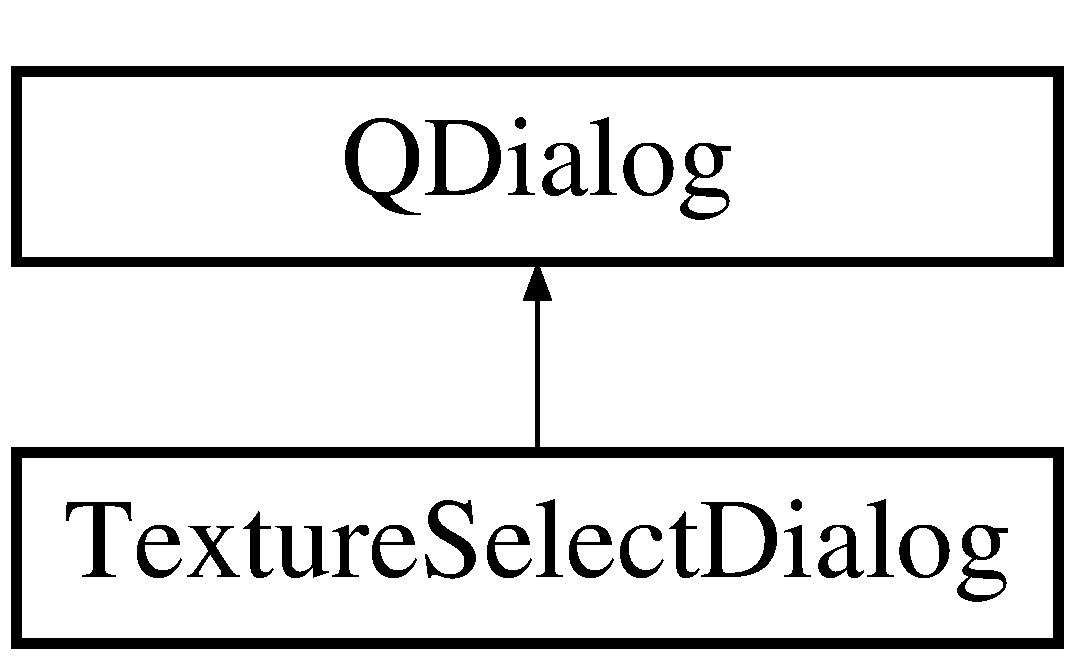
\includegraphics[height=2.000000cm]{class_texture_select_dialog}
\end{center}
\end{figure}
\subsection*{Public Member Functions}
\begin{DoxyCompactItemize}
\item 
\hyperlink{class_texture_select_dialog_a76784e782a28dd37c8739cd93a77ee95}{Texture\+Select\+Dialog} (\hyperlink{class_texture_handler}{Texture\+Handler} $\ast$texture\+Handler, Q\+Widget $\ast$parent=0)
\begin{DoxyCompactList}\small\item\em Constructeur de base de la fenêtre \hyperlink{class_texture_select_dialog}{Texture\+Select\+Dialog}. \end{DoxyCompactList}\item 
\hyperlink{class_texture_select_dialog_afa8268eacb42fa8ff6b6372e7a8da9fd}{$\sim$\+Texture\+Select\+Dialog} ()
\item 
int \hyperlink{class_texture_select_dialog_aac9d46bff08b03776e5da51ffe5e8527}{selected\+Texture\+Index} () const 
\begin{DoxyCompactList}\small\item\em Getter. \end{DoxyCompactList}\end{DoxyCompactItemize}


\subsection{Detailed Description}
Classe de fenêtre de sélection de texture. 

\begin{DoxyAuthor}{Author}
Valentin D.\+d.\+G. 
\end{DoxyAuthor}
\begin{DoxyVersion}{Version}
1.\+0
\end{DoxyVersion}
En fonction du gestionnaire de texture passé en paramètre, la fenêtre affiche les textures que le gestionnaire contient et les affiche en forme de liste. Lorsque la fenêtre se ferme, il est possible de récupérer l\textquotesingle{}index de la dernière texture sélectionnée via la fonction selected\+Texture\+Index. 

\subsection{Constructor \& Destructor Documentation}
\hypertarget{class_texture_select_dialog_a76784e782a28dd37c8739cd93a77ee95}{}\index{Texture\+Select\+Dialog@{Texture\+Select\+Dialog}!Texture\+Select\+Dialog@{Texture\+Select\+Dialog}}
\index{Texture\+Select\+Dialog@{Texture\+Select\+Dialog}!Texture\+Select\+Dialog@{Texture\+Select\+Dialog}}
\subsubsection[{Texture\+Select\+Dialog(\+Texture\+Handler $\ast$texture\+Handler, Q\+Widget $\ast$parent=0)}]{\setlength{\rightskip}{0pt plus 5cm}Texture\+Select\+Dialog\+::\+Texture\+Select\+Dialog (
\begin{DoxyParamCaption}
\item[{{\bf Texture\+Handler} $\ast$}]{texture\+Handler, }
\item[{Q\+Widget $\ast$}]{parent = {\ttfamily 0}}
\end{DoxyParamCaption}
)\hspace{0.3cm}{\ttfamily [explicit]}}\label{class_texture_select_dialog_a76784e782a28dd37c8739cd93a77ee95}


Constructeur de base de la fenêtre \hyperlink{class_texture_select_dialog}{Texture\+Select\+Dialog}. 


\begin{DoxyParams}{Parameters}
{\em texture\+Handler} & Gestionnaire de texture que la fenêtre liste. \\
\hline
{\em parent} & Parent de la fenêtre. \\
\hline
\end{DoxyParams}
\hypertarget{class_texture_select_dialog_afa8268eacb42fa8ff6b6372e7a8da9fd}{}\index{Texture\+Select\+Dialog@{Texture\+Select\+Dialog}!````~Texture\+Select\+Dialog@{$\sim$\+Texture\+Select\+Dialog}}
\index{````~Texture\+Select\+Dialog@{$\sim$\+Texture\+Select\+Dialog}!Texture\+Select\+Dialog@{Texture\+Select\+Dialog}}
\subsubsection[{$\sim$\+Texture\+Select\+Dialog()}]{\setlength{\rightskip}{0pt plus 5cm}Texture\+Select\+Dialog\+::$\sim$\+Texture\+Select\+Dialog (
\begin{DoxyParamCaption}
{}
\end{DoxyParamCaption}
)}\label{class_texture_select_dialog_afa8268eacb42fa8ff6b6372e7a8da9fd}
Destructeur de \hyperlink{class_texture_select_dialog}{Texture\+Select\+Dialog}. 

\subsection{Member Function Documentation}
\hypertarget{class_texture_select_dialog_aac9d46bff08b03776e5da51ffe5e8527}{}\index{Texture\+Select\+Dialog@{Texture\+Select\+Dialog}!selected\+Texture\+Index@{selected\+Texture\+Index}}
\index{selected\+Texture\+Index@{selected\+Texture\+Index}!Texture\+Select\+Dialog@{Texture\+Select\+Dialog}}
\subsubsection[{selected\+Texture\+Index() const }]{\setlength{\rightskip}{0pt plus 5cm}int Texture\+Select\+Dialog\+::selected\+Texture\+Index (
\begin{DoxyParamCaption}
{}
\end{DoxyParamCaption}
) const}\label{class_texture_select_dialog_aac9d46bff08b03776e5da51ffe5e8527}


Getter. 

\begin{DoxyReturn}{Returns}
Index de la dernière texture sélectionnée. 
\end{DoxyReturn}


The documentation for this class was generated from the following files\+:\begin{DoxyCompactItemize}
\item 
textureselectdialog.\+h\item 
textureselectdialog.\+cpp\end{DoxyCompactItemize}

\hypertarget{struct_unit_data__str}{}\section{Unit\+Data\+\_\+str Struct Reference}
\label{struct_unit_data__str}\index{Unit\+Data\+\_\+str@{Unit\+Data\+\_\+str}}


Petite structure regroupant les paramètres principaux d\textquotesingle{}une unité.  




{\ttfamily \#include $<$editorlevel.\+h$>$}

\subsection*{Public Attributes}
\begin{DoxyCompactItemize}
\item 
\hypertarget{struct_unit_data__str_ae3043d1b98cdd975c3bb3d409e4fff94}{}Q\+Point \hyperlink{struct_unit_data__str_ae3043d1b98cdd975c3bb3d409e4fff94}{position}\label{struct_unit_data__str_ae3043d1b98cdd975c3bb3d409e4fff94}

\begin{DoxyCompactList}\small\item\em Position de l\textquotesingle{}unité. \end{DoxyCompactList}\item 
\hypertarget{struct_unit_data__str_a45215b0d49d28d3eeb883cd8e655cf3e}{}bool \hyperlink{struct_unit_data__str_a45215b0d49d28d3eeb883cd8e655cf3e}{halfx}\label{struct_unit_data__str_a45215b0d49d28d3eeb883cd8e655cf3e}

\begin{DoxyCompactList}\small\item\em Si vrai, la position est décalé d\textquotesingle{}une demi case vers la droite. \end{DoxyCompactList}\item 
\hypertarget{struct_unit_data__str_a1c885dc06eb76926b95a1ecad73a7f4a}{}bool \hyperlink{struct_unit_data__str_a1c885dc06eb76926b95a1ecad73a7f4a}{halfy}\label{struct_unit_data__str_a1c885dc06eb76926b95a1ecad73a7f4a}

\begin{DoxyCompactList}\small\item\em Si vrai, la position est décalé d\textquotesingle{}une demi case vers le bas. \end{DoxyCompactList}\item 
\hypertarget{struct_unit_data__str_a0189b64bcee5c40ddbff6b1b53cb5282}{}int \hyperlink{struct_unit_data__str_a0189b64bcee5c40ddbff6b1b53cb5282}{speed}\label{struct_unit_data__str_a0189b64bcee5c40ddbff6b1b53cb5282}

\begin{DoxyCompactList}\small\item\em Vitesse normale de l\textquotesingle{}unité. \end{DoxyCompactList}\item 
\hypertarget{struct_unit_data__str_a328dbd260b3684372a61ff434347796f}{}int \hyperlink{struct_unit_data__str_a328dbd260b3684372a61ff434347796f}{sspeed}\label{struct_unit_data__str_a328dbd260b3684372a61ff434347796f}

\begin{DoxyCompactList}\small\item\em Vitesse de l\textquotesingle{}unité lorsque les fantômes sont appeurés. \end{DoxyCompactList}\end{DoxyCompactItemize}


\subsection{Detailed Description}
Petite structure regroupant les paramètres principaux d\textquotesingle{}une unité. 

The documentation for this struct was generated from the following file\+:\begin{DoxyCompactItemize}
\item 
editorlevel.\+h\end{DoxyCompactItemize}

\hypertarget{structunit_widget_set__str}{}\section{unit\+Widget\+Set\+\_\+str Struct Reference}
\label{structunit_widget_set__str}\index{unit\+Widget\+Set\+\_\+str@{unit\+Widget\+Set\+\_\+str}}


Structure contenant les objets d\textquotesingle{}interface lié à une unité.  




{\ttfamily \#include $<$mainwindow.\+h$>$}

\subsection*{Public Attributes}
\begin{DoxyCompactItemize}
\item 
\hypertarget{structunit_widget_set__str_a434e160dda006f11ae717fee0718e0b7}{}Q\+Spin\+Box $\ast$ \hyperlink{structunit_widget_set__str_a434e160dda006f11ae717fee0718e0b7}{speed}\label{structunit_widget_set__str_a434e160dda006f11ae717fee0718e0b7}

\begin{DoxyCompactList}\small\item\em Spin\+Box réglant la vitesse. \end{DoxyCompactList}\item 
\hypertarget{structunit_widget_set__str_a72acd0e89c9f4a2128ccad7054a235f6}{}Q\+Spin\+Box $\ast$ \hyperlink{structunit_widget_set__str_a72acd0e89c9f4a2128ccad7054a235f6}{sspeed}\label{structunit_widget_set__str_a72acd0e89c9f4a2128ccad7054a235f6}

\begin{DoxyCompactList}\small\item\em Spin\+Box réglant la vitesse lors du mode Appeuré. \end{DoxyCompactList}\item 
\hypertarget{structunit_widget_set__str_a174d84c9d3802e2cc121d7f5a45ec730}{}Q\+Spin\+Box $\ast$ \hyperlink{structunit_widget_set__str_a174d84c9d3802e2cc121d7f5a45ec730}{posx}\label{structunit_widget_set__str_a174d84c9d3802e2cc121d7f5a45ec730}

\begin{DoxyCompactList}\small\item\em Spin\+Box réglant la position en largeur. \end{DoxyCompactList}\item 
\hypertarget{structunit_widget_set__str_a384ea3590f9ce6094295c813c9db0a17}{}Q\+Spin\+Box $\ast$ \hyperlink{structunit_widget_set__str_a384ea3590f9ce6094295c813c9db0a17}{posy}\label{structunit_widget_set__str_a384ea3590f9ce6094295c813c9db0a17}

\begin{DoxyCompactList}\small\item\em Spin\+Box réglant la position en hauteur. \end{DoxyCompactList}\item 
\hypertarget{structunit_widget_set__str_aab1c1c43fafcd7062fa8cfd4136a30b6}{}Q\+Check\+Box $\ast$ \hyperlink{structunit_widget_set__str_aab1c1c43fafcd7062fa8cfd4136a30b6}{halfx}\label{structunit_widget_set__str_aab1c1c43fafcd7062fa8cfd4136a30b6}

\begin{DoxyCompactList}\small\item\em Case à cocher réglant l\textquotesingle{}offset d\textquotesingle{}une demi-\/case en largeur. \end{DoxyCompactList}\item 
\hypertarget{structunit_widget_set__str_a7ff01fa2c0ada654b42896842a0ab5f4}{}Q\+Check\+Box $\ast$ \hyperlink{structunit_widget_set__str_a7ff01fa2c0ada654b42896842a0ab5f4}{halfy}\label{structunit_widget_set__str_a7ff01fa2c0ada654b42896842a0ab5f4}

\begin{DoxyCompactList}\small\item\em Case à cocher réglant l\textquotesingle{}offset d\textquotesingle{}une demi-\/case en hauteur. \end{DoxyCompactList}\end{DoxyCompactItemize}


\subsection{Detailed Description}
Structure contenant les objets d\textquotesingle{}interface lié à une unité. 

The documentation for this struct was generated from the following file\+:\begin{DoxyCompactItemize}
\item 
mainwindow.\+h\end{DoxyCompactItemize}

\hypertarget{class_view}{}\section{View Class Reference}
\label{class_view}\index{View@{View}}


Classe graphique remplaçant la vue de Qt pour propager les événements.  




{\ttfamily \#include $<$view.\+h$>$}

Inheritance diagram for View\+:\begin{figure}[H]
\begin{center}
\leavevmode
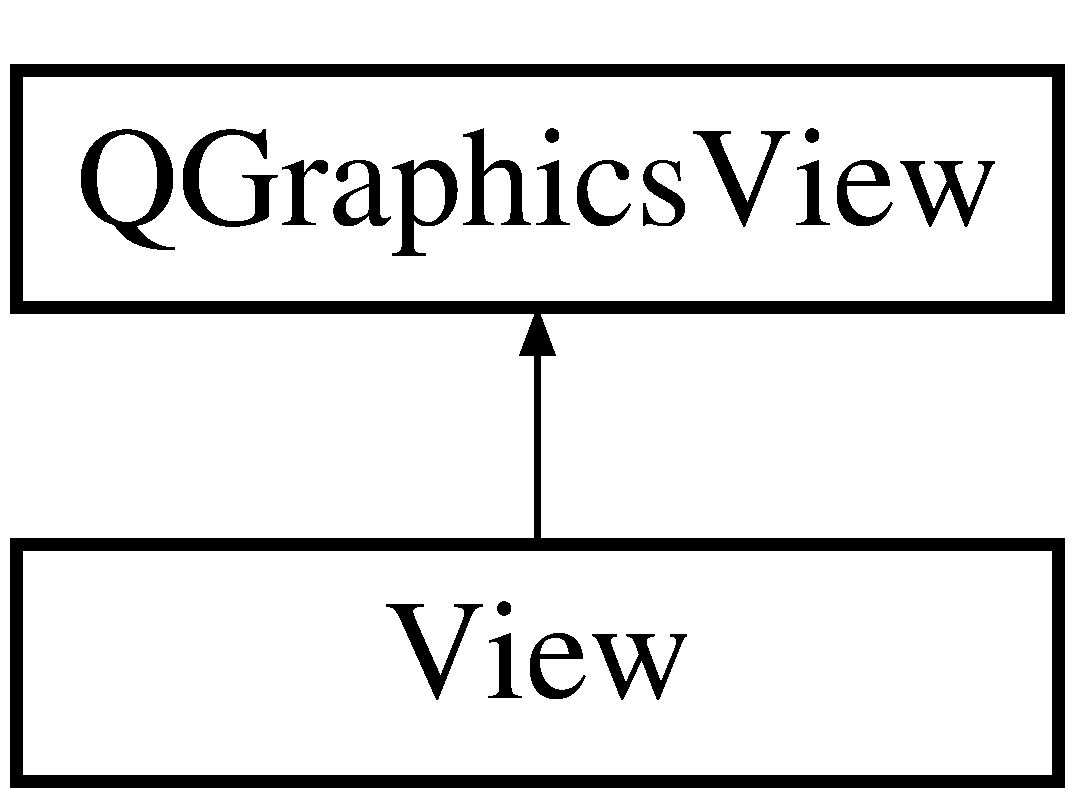
\includegraphics[height=2.000000cm]{class_view}
\end{center}
\end{figure}
\subsection*{Signals}
\begin{DoxyCompactItemize}
\item 
void \hyperlink{class_view_ac62e4287149000223df6f3608555c93a}{wheel\+Event\+On\+View} (Q\+Wheel\+Event $\ast$event)
\begin{DoxyCompactList}\small\item\em Signal émit lors de l\textquotesingle{}événement de molette de la souris. \end{DoxyCompactList}\end{DoxyCompactItemize}
\subsection*{Public Member Functions}
\begin{DoxyCompactItemize}
\item 
\hyperlink{class_view_a74d64dd513eae96bc3196131f865a4e8}{View} (Q\+Widget $\ast$parent=0)
\begin{DoxyCompactList}\small\item\em Constructeur de base de \hyperlink{class_view}{View}. \end{DoxyCompactList}\item 
\hyperlink{class_view_ad0dc854db9aabbea98a334dec89f785c}{$\sim$\+View} ()
\end{DoxyCompactItemize}
\subsection*{Protected Member Functions}
\begin{DoxyCompactItemize}
\item 
void \hyperlink{class_view_ae10a826d1ff69353664c4ffc0accc039}{wheel\+Event} (Q\+Wheel\+Event $\ast$event)
\begin{DoxyCompactList}\small\item\em Surchage de la fonction d\textquotesingle{}événement de molette de la souris. \end{DoxyCompactList}\end{DoxyCompactItemize}


\subsection{Detailed Description}
Classe graphique remplaçant la vue de Qt pour propager les événements. 

\begin{DoxyAuthor}{Author}
Valentin D.\+d.\+G. 
\end{DoxyAuthor}
\begin{DoxyVersion}{Version}
1.\+0
\end{DoxyVersion}
La classe \hyperlink{class_view}{View} propage les événements de molette de souris avec le signal wheel\+Event\+On\+View. 

\subsection{Constructor \& Destructor Documentation}
\hypertarget{class_view_a74d64dd513eae96bc3196131f865a4e8}{}\index{View@{View}!View@{View}}
\index{View@{View}!View@{View}}
\subsubsection[{View(\+Q\+Widget $\ast$parent=0)}]{\setlength{\rightskip}{0pt plus 5cm}View\+::\+View (
\begin{DoxyParamCaption}
\item[{Q\+Widget $\ast$}]{parent = {\ttfamily 0}}
\end{DoxyParamCaption}
)}\label{class_view_a74d64dd513eae96bc3196131f865a4e8}


Constructeur de base de \hyperlink{class_view}{View}. 


\begin{DoxyParams}{Parameters}
{\em parent} & Parent de la fenêtre. \\
\hline
\end{DoxyParams}
\hypertarget{class_view_ad0dc854db9aabbea98a334dec89f785c}{}\index{View@{View}!````~View@{$\sim$\+View}}
\index{````~View@{$\sim$\+View}!View@{View}}
\subsubsection[{$\sim$\+View()}]{\setlength{\rightskip}{0pt plus 5cm}View\+::$\sim$\+View (
\begin{DoxyParamCaption}
{}
\end{DoxyParamCaption}
)}\label{class_view_ad0dc854db9aabbea98a334dec89f785c}
Destructeur de \hyperlink{class_view}{View}. 

\subsection{Member Function Documentation}
\hypertarget{class_view_ae10a826d1ff69353664c4ffc0accc039}{}\index{View@{View}!wheel\+Event@{wheel\+Event}}
\index{wheel\+Event@{wheel\+Event}!View@{View}}
\subsubsection[{wheel\+Event(\+Q\+Wheel\+Event $\ast$event)}]{\setlength{\rightskip}{0pt plus 5cm}void View\+::wheel\+Event (
\begin{DoxyParamCaption}
\item[{Q\+Wheel\+Event $\ast$}]{event}
\end{DoxyParamCaption}
)\hspace{0.3cm}{\ttfamily [protected]}}\label{class_view_ae10a826d1ff69353664c4ffc0accc039}


Surchage de la fonction d\textquotesingle{}événement de molette de la souris. 


\begin{DoxyParams}{Parameters}
{\em event} & Paramètre généré par l\textquotesingle{}événement. \\
\hline
\end{DoxyParams}
\hypertarget{class_view_ac62e4287149000223df6f3608555c93a}{}\index{View@{View}!wheel\+Event\+On\+View@{wheel\+Event\+On\+View}}
\index{wheel\+Event\+On\+View@{wheel\+Event\+On\+View}!View@{View}}
\subsubsection[{wheel\+Event\+On\+View}]{\setlength{\rightskip}{0pt plus 5cm}void View\+::wheel\+Event\+On\+View (
\begin{DoxyParamCaption}
\item[{Q\+Wheel\+Event $\ast$}]{event}
\end{DoxyParamCaption}
)\hspace{0.3cm}{\ttfamily [signal]}}\label{class_view_ac62e4287149000223df6f3608555c93a}


Signal émit lors de l\textquotesingle{}événement de molette de la souris. 


\begin{DoxyParams}{Parameters}
{\em event} & Paramètre généré par l\textquotesingle{}événement. \\
\hline
\end{DoxyParams}


The documentation for this class was generated from the following files\+:\begin{DoxyCompactItemize}
\item 
view.\+h\item 
view.\+cpp\end{DoxyCompactItemize}

%--- End generated contents ---

% Index
\backmatter
\newpage
\phantomsection
\clearemptydoublepage
\addcontentsline{toc}{chapter}{Index}
\printindex

\end{document}
